% Options for packages loaded elsewhere
\PassOptionsToPackage{unicode}{hyperref}
\PassOptionsToPackage{hyphens}{url}
%
\documentclass[
]{article}
\usepackage{amsmath,amssymb}
\usepackage{iftex}
\ifPDFTeX
  \usepackage[T1]{fontenc}
  \usepackage[utf8]{inputenc}
  \usepackage{textcomp} % provide euro and other symbols
\else % if luatex or xetex
  \usepackage{unicode-math} % this also loads fontspec
  \defaultfontfeatures{Scale=MatchLowercase}
  \defaultfontfeatures[\rmfamily]{Ligatures=TeX,Scale=1}
\fi
\usepackage{lmodern}
\ifPDFTeX\else
  % xetex/luatex font selection
\fi
% Use upquote if available, for straight quotes in verbatim environments
\IfFileExists{upquote.sty}{\usepackage{upquote}}{}
\IfFileExists{microtype.sty}{% use microtype if available
  \usepackage[]{microtype}
  \UseMicrotypeSet[protrusion]{basicmath} % disable protrusion for tt fonts
}{}
\makeatletter
\@ifundefined{KOMAClassName}{% if non-KOMA class
  \IfFileExists{parskip.sty}{%
    \usepackage{parskip}
  }{% else
    \setlength{\parindent}{0pt}
    \setlength{\parskip}{6pt plus 2pt minus 1pt}}
}{% if KOMA class
  \KOMAoptions{parskip=half}}
\makeatother
\usepackage{xcolor}
\usepackage[margin=1in]{geometry}
\usepackage{color}
\usepackage{fancyvrb}
\newcommand{\VerbBar}{|}
\newcommand{\VERB}{\Verb[commandchars=\\\{\}]}
\DefineVerbatimEnvironment{Highlighting}{Verbatim}{commandchars=\\\{\}}
% Add ',fontsize=\small' for more characters per line
\usepackage{framed}
\definecolor{shadecolor}{RGB}{248,248,248}
\newenvironment{Shaded}{\begin{snugshade}}{\end{snugshade}}
\newcommand{\AlertTok}[1]{\textcolor[rgb]{0.94,0.16,0.16}{#1}}
\newcommand{\AnnotationTok}[1]{\textcolor[rgb]{0.56,0.35,0.01}{\textbf{\textit{#1}}}}
\newcommand{\AttributeTok}[1]{\textcolor[rgb]{0.13,0.29,0.53}{#1}}
\newcommand{\BaseNTok}[1]{\textcolor[rgb]{0.00,0.00,0.81}{#1}}
\newcommand{\BuiltInTok}[1]{#1}
\newcommand{\CharTok}[1]{\textcolor[rgb]{0.31,0.60,0.02}{#1}}
\newcommand{\CommentTok}[1]{\textcolor[rgb]{0.56,0.35,0.01}{\textit{#1}}}
\newcommand{\CommentVarTok}[1]{\textcolor[rgb]{0.56,0.35,0.01}{\textbf{\textit{#1}}}}
\newcommand{\ConstantTok}[1]{\textcolor[rgb]{0.56,0.35,0.01}{#1}}
\newcommand{\ControlFlowTok}[1]{\textcolor[rgb]{0.13,0.29,0.53}{\textbf{#1}}}
\newcommand{\DataTypeTok}[1]{\textcolor[rgb]{0.13,0.29,0.53}{#1}}
\newcommand{\DecValTok}[1]{\textcolor[rgb]{0.00,0.00,0.81}{#1}}
\newcommand{\DocumentationTok}[1]{\textcolor[rgb]{0.56,0.35,0.01}{\textbf{\textit{#1}}}}
\newcommand{\ErrorTok}[1]{\textcolor[rgb]{0.64,0.00,0.00}{\textbf{#1}}}
\newcommand{\ExtensionTok}[1]{#1}
\newcommand{\FloatTok}[1]{\textcolor[rgb]{0.00,0.00,0.81}{#1}}
\newcommand{\FunctionTok}[1]{\textcolor[rgb]{0.13,0.29,0.53}{\textbf{#1}}}
\newcommand{\ImportTok}[1]{#1}
\newcommand{\InformationTok}[1]{\textcolor[rgb]{0.56,0.35,0.01}{\textbf{\textit{#1}}}}
\newcommand{\KeywordTok}[1]{\textcolor[rgb]{0.13,0.29,0.53}{\textbf{#1}}}
\newcommand{\NormalTok}[1]{#1}
\newcommand{\OperatorTok}[1]{\textcolor[rgb]{0.81,0.36,0.00}{\textbf{#1}}}
\newcommand{\OtherTok}[1]{\textcolor[rgb]{0.56,0.35,0.01}{#1}}
\newcommand{\PreprocessorTok}[1]{\textcolor[rgb]{0.56,0.35,0.01}{\textit{#1}}}
\newcommand{\RegionMarkerTok}[1]{#1}
\newcommand{\SpecialCharTok}[1]{\textcolor[rgb]{0.81,0.36,0.00}{\textbf{#1}}}
\newcommand{\SpecialStringTok}[1]{\textcolor[rgb]{0.31,0.60,0.02}{#1}}
\newcommand{\StringTok}[1]{\textcolor[rgb]{0.31,0.60,0.02}{#1}}
\newcommand{\VariableTok}[1]{\textcolor[rgb]{0.00,0.00,0.00}{#1}}
\newcommand{\VerbatimStringTok}[1]{\textcolor[rgb]{0.31,0.60,0.02}{#1}}
\newcommand{\WarningTok}[1]{\textcolor[rgb]{0.56,0.35,0.01}{\textbf{\textit{#1}}}}
\usepackage{graphicx}
\makeatletter
\def\maxwidth{\ifdim\Gin@nat@width>\linewidth\linewidth\else\Gin@nat@width\fi}
\def\maxheight{\ifdim\Gin@nat@height>\textheight\textheight\else\Gin@nat@height\fi}
\makeatother
% Scale images if necessary, so that they will not overflow the page
% margins by default, and it is still possible to overwrite the defaults
% using explicit options in \includegraphics[width, height, ...]{}
\setkeys{Gin}{width=\maxwidth,height=\maxheight,keepaspectratio}
% Set default figure placement to htbp
\makeatletter
\def\fps@figure{htbp}
\makeatother
\setlength{\emergencystretch}{3em} % prevent overfull lines
\providecommand{\tightlist}{%
  \setlength{\itemsep}{0pt}\setlength{\parskip}{0pt}}
\setcounter{secnumdepth}{-\maxdimen} % remove section numbering
\usepackage{booktabs}
\usepackage{longtable}
\usepackage{array}
\usepackage{multirow}
\usepackage{wrapfig}
\usepackage{float}
\usepackage{colortbl}
\usepackage{pdflscape}
\usepackage{tabu}
\usepackage{threeparttable}
\usepackage{threeparttablex}
\usepackage[normalem]{ulem}
\usepackage{makecell}
\usepackage{xcolor}
\ifLuaTeX
  \usepackage{selnolig}  % disable illegal ligatures
\fi
\usepackage{bookmark}
\IfFileExists{xurl.sty}{\usepackage{xurl}}{} % add URL line breaks if available
\urlstyle{same}
\hypersetup{
  hidelinks,
  pdfcreator={LaTeX via pandoc}}

\author{}
\date{\vspace{-2.5em}}

\begin{document}

\section{Fundamentals of Data Science Assessment
Sheet}\label{fundamentals-of-data-science-assessment-sheet}

\paragraph{\texorpdfstring{\emph{Matt
Prill}}{Matt Prill}}\label{matt-prill}

Note: \emph{Version control has been used to track my workflow and all
these documents are accessible through my github repository
\href{https://github.com/prillex/fundamental_assessed_exercises}{linked
here}. It also contains images of my hand written workings out. My
workflow for the R questions can be found in the `rough\_workflow.R'
file. There is no onus to look at these; all relevant and neat workings
can be seen in this document. I have included them in the repository to
(A) track my own workflow (version control) and (B) allow you to consult
them should you wish to.}

\subsection{Question 1a}\label{question-1a}

\paragraph{Initial Equations:}\label{initial-equations}

\[
\Large
\begin{aligned}
x + y + z &= 1 \\
x + 2y + 4z &= \eta \\
x + 4y + 10z &= \eta^2
\end{aligned}
\]\\

\paragraph{Corresponding Coefficient
Matrix:}\label{corresponding-coefficient-matrix}

\[
\Large
A = \begin{bmatrix}
1 & 1 & 1 \\
1 & 2 & 4 \\
1 & 4 & 10 
\end{bmatrix}
\begin{bmatrix}
1  \\
η  \\
η^2  
\end{bmatrix}
\]

\paragraph{Calculating the Determinant of
A:}\label{calculating-the-determinant-of-a}

To showcase that these equations lack a unique solution for any value of
η, I can attempt to find the determinant. To to find a determinant of
square matrix (irrespective of size), I must;

\begin{enumerate}
\def\labelenumi{\arabic{enumi}.}
\tightlist
\item
  Pick a coefficient from the first row.
\item
  Delete remaining elements in coefficient's respective row and column.
\item
  Make a matrix of the remaining elements.
\item
  Find the determinant of the sub-matrix, and multiply this with the
  coefficient.
\item
  Repeat the same procedure for each element in the first row.
\item
  To determine the sign of each term, sum the indices of the
  coefficient. If it is even, the sign is positive, and if it's odd, the
  sign is negative.
\item
  Sum all terms to find the determinant.
\end{enumerate}

Therefore, to find the determinant (\(\text{det}\)) of a \(3 \times 3\)
matrix, I can use the following formula:

\[
\Large
\text{det} \begin{bmatrix} a & b & c \\ d & e & f \\ g & h & i \end{bmatrix} = a \times \text{det} \begin{bmatrix} e & f \\ h & i \end{bmatrix} - b \times \text{det} \begin{bmatrix} d & f \\ g & i \end{bmatrix} + c \times \text{det} \begin{bmatrix} d & e \\ g & h \end{bmatrix}
\]

The terms are added/ subtracted depending on the sum the row and column
indices of the coefficient. Even = positive. Odd = negative. For example
``- b'' is negative because b is \(x_{12}\), thus the sum of the row and
column indices \(= 1+2 = 3 = odd\).

Applying this to the \(3 \times 3\) matrix:

\[
\Large
A = \begin{bmatrix}
1 & 1 & 1 \\
1 & 2 & 4 \\
1 & 4 & 10 
\end{bmatrix}
=
\begin{bmatrix}
a & b & c \\
d & e & f \\
g & h & i 
\end{bmatrix}
\]

Thus,

\[
\Large
\text{det}(A) =
1 \times \text{det} \begin{bmatrix} 2 & 4 \\ 4 & 10 \end{bmatrix} - 1 \times \text{det} \begin{bmatrix} 1 & 4 \\ 1 & 10 \end{bmatrix} + 1 \times \text{det} \begin{bmatrix} 1 & 2 \\ 1 & 4 \end{bmatrix}
\]

To calculate the determinants of the \(2 \times 2\) matrices, I can
apply the formula:

\[
\Large
\text{det}\begin{bmatrix} a & b \\ c & d \end{bmatrix} = ad - bc
\]

Corresponding calculations for determinants of the \(2 \times 2\)
matrices:

\[
\Large
\text{det} 
 \begin{bmatrix} 2 & 4 \\ 4 & 10 \end{bmatrix} = 20 - 16 =\mathbf{4}
\]

\[
\Large
 \text{det} \begin{bmatrix} 1 & 4 \\ 1 & 10 \end{bmatrix} = 10 - 4 =\mathbf{6}
\]

\[
\Large
 \text{det} \begin{bmatrix} 1 & 2 \\ 1 & 4 \end{bmatrix} = 4-2 = \mathbf{2}
\]

Substituting these determinants into the aforementioned \(3 \times 3\)
matrix determinant formula gives:

\[
\Large
\text{det}(A)=
(1 \times 4)  - (1 \times 6) + (1 \times 2) = \mathbf{0}
\]

The determinant of the coefficient matrix and therefore the matrix
vector is \(0\). This means that the matrix is singular:

\[
\Large
\text{det}(A) = Ax = 0
\]\\

In being singular, the matrix does not have an inverse meaning that the
corresponding linear equations have either no, or unlimited solutions.
Regardless, in this case, the initial equations have no unique solution
for \(η\).

\hfill\break
\hfill\break
\hfill\break
\hfill\break

\subsection{Question 1b}\label{question-1b}

\paragraph{The Set of Linear
Equations:}\label{the-set-of-linear-equations}

\[
\Large
\begin{aligned}
x + y + z &= 1 \\
x + 2y + 4z &= \eta \\
x + 4y + 10z &= \eta^2
\end{aligned}
\]\\

\paragraph{The Corresponding Augmented
Matrix:}\label{the-corresponding-augmented-matrix}

\[
\Large
\left[
\begin{array}{ccc|c}
1 & 1 & 1 & 1 \\
1 & 2 & 4 & \eta \\
1 & 4 & 10 & \eta^2
\end{array}
\right]
\]

\paragraph{Using Gaussian Elimination to Identify the Solutions for
η:}\label{using-gaussian-elimination-to-identify-the-solutions-for-ux3b7}

\begin{enumerate}
\def\labelenumi{\arabic{enumi}.}
\item
  \[\Large
  (\text{Row }2) -1 \times (1) = 
  \left[
  \begin{array}{ccc|c}
  1 & 1 & 1 & 1 \\
  0 & 1 & 3 & \eta-1 \\
  1 & 4 & 10 & \eta^2
  \end{array}
  \right]
  \]
\item
  \[\Large
   (\text{Row } 3) -1 \times (1) = 
  \left[
  \begin{array}{ccc|c}
  1 & 1 & 1 & 1 \\
  0 & 1 & 3 & \eta-1 \\
  0 & 3 & 9 & \eta^2-1
  \end{array}
  \right]
  \]
\item
  \[\Large
  (\text{Row }3) -3 \times (2) = 
  \left[
  \begin{array}{ccc|c}
  1 & 1 & 1 & 1 \\
  0 & 1 & 3 & \eta-1 \\
  0 & 0 & 0 & \eta^2-3\eta +2
  \end{array}
  \right]
  \]\\
\end{enumerate}

The equation corresponding to the bottom row of the augmented matrix is
0. It is also a quadratic equation where:

\[
\Large
\eta^2-3\eta +2
= ax^2 + bx + c = 0
\]

Now, I can either factorise:

\[
\Large
\eta^2-3\eta +2=
(\eta-1)(\eta-2)= 0
\]

Or alternatively, I can use the quadratic formula to derive the
solutions for \(\eta\):

\[
\Large
\eta = \frac{-b \pm \sqrt{b^2 - 4ac}}{2a}
 = \frac{-(-3) \pm \sqrt{-3^2 - 4\times1\times2}}{2\times1}
 = 1 \text{ or } 2
\]

\hfill\break

\[
\Large
\eta = 1 \text{ or } 2
\]

\hfill\break

\paragraph{Characterising the equations for both
solutions:}\label{characterising-the-equations-for-both-solutions}

\subparagraph{\texorpdfstring{Where
\(\eta = 1\):}{Where \textbackslash eta = 1:}}\label{where-eta-1}

\[
\Large
\begin{aligned}
x + y + z &= 1 \\
x + 2y + 4z &= 1 \\
x + 4y + 10z &= 1^2
\end{aligned}
\]

Corresponding augmented matrix:

\[
\Large
\left[
\begin{array}{ccc|c}
1 & 1 & 1 & 1 \\
0 & 1 & 3 & 1-1 \\
0 & 0 & 0 & 1^2-3(1)\ + 2
\end{array}
\right]
\Large
= 
\left[
\begin{array}{ccc|c}
1 & 1 & 1 & 1 \\
0 & 1 & 3 & 0 \\
0 & 0 & 0 & 0\ 
\end{array}
\right]
\]

Thus, when \(\eta = 1\):

\[
\Large
\begin{aligned}
x + y + z &= 1 \\
y + 3z & = 0 \\
\end{aligned}
\]

\subsection{?Now I can assign the free variable (z) to a parameter and
characterise
?}\label{now-i-can-assign-the-free-variable-z-to-a-parameter-and-characterise}

\hfill\break
\hfill\break
\hfill\break

\subparagraph{\texorpdfstring{Where
\(\eta = 2\):}{Where \textbackslash eta = 2:}}\label{where-eta-2}

\[
\Large
\begin{aligned}
x + y + z &= 1 \\
x + 2y + 4z &= 2 \\
x + 4y + 10z &= 2^2
\end{aligned}
\]

Corresponding augmented matrix:

\[
\Large
\left[
\begin{array}{ccc|c}
1 & 1 & 1 & 1 \\
0 & 1 & 3 & 2-1 \\
0 & 0 & 0 & 2^2-3(2)\ + 2
\end{array}
\right]
\Large
= 
\left[
\begin{array}{ccc|c}
1 & 1 & 1 & 1 \\
0 & 1 & 3 & 1 \\
0 & 0 & 0 & 0\ 
\end{array}
\right]
\]

Thus when \(\eta = 2\):

\[
\Large
\begin{aligned}
x + y + z &= 1 \\
y + 3z & = 1 \\
\end{aligned}
\]

\subsection{?Now I can assign the free variable (z) to a parameter and
characterise?}\label{now-i-can-assign-the-free-variable-z-to-a-parameter-and-characterise-1}

\hfill\break
\hfill\break
\hfill\break
\hfill\break
\hfill\break
\hfill\break

\subsection{Question 2a}\label{question-2a}

\(P_{1} = P(\text{Alice winning when first to throw})\)

The distribution shares some characteristics of the Bernoulli
distribution whereby there are two outcomes (success \& failure) and
discrete. However, the question is asking for the probability to a given
success. The balls are thrown (trials) until a success (hit).
Furthermore, I have to assume that each throw is independent of the
other which makes the distribution memoryless with two outcomes: success
(win), \& failure (miss). This is a geometric distribution.

\[
\large
\left.
\begin{aligned}
\text{Hit} = α\\
\text{Miss}= 1-α\
\end{aligned}
\right\} \text{Alice}
\]

\[
\large
\left.
\begin{aligned}
\text{Hit} =  β\\
\text{Miss}= 1- β\
\end{aligned}
\right\} \text{Ben}
\]

\paragraph{The probability of Alice missing Ben with her first throw and
going on to
win:}\label{the-probability-of-alice-missing-ben-with-her-first-throw-and-going-on-to-win}

P(Alice misses first throw) = \(1 - α\)

P(Ben misses first throw) = \(1-β\)

Thus,\\
P(Alice miss, Ben miss) = \((1 - α)\times (1-β)\)

So,\\
P(Alice miss, Ben miss, Alice goes onto win) =
\(P_{1}\times(1 - α) \times(1 - β)\)

\(P_{1}\) is able to be used here because of the memoryless nature of
the geometric distribution; no matter how many trials have transpired
prior to a given throw of Alice's, the probability that she will win
from that point onwards is still \(P_{1}\).

\hfill\break
\hfill\break

\subsection{Question 2b}\label{question-2b}

Because I'm working with the Geometric distribution with parameter p, X
has a probability mass function:

\[
\large
P(X = k) = p(k) =
\left\{
\begin{aligned}
(1 − p)^{k-1}p,\\
0\
\end{aligned}
\right.
\]

This is not conditional probability as the probability is with respect
to the beginning of the round.

As discussed, the probability that Alice and Ben both miss in a given
round is: \((1 - α)\times (1-β)\)

\hfill\break
This could repeat n times where n can denotes any integer
(theoretically): \(((1 - α)\times (1-β))^n\) meaning the probability
will be a summation of all the rounds where n is potentially indefinite
\((\sum_{n=1}^{\infty})\)

\hfill\break
Eventual success from Alice (given that she throws first) therefore
gives: \[
\Large
P(X = n) =  \sum_{n=1}^{\infty} ((1 - α)\times (1-β))^{n-1} \timesα
\]\\

The \(n-1\) term is used because Alice and Ben must miss every time
until the final round (hence \(-1\)); the \(n\)-th round is the one she
wins (success).

The \(α\) term is therefore added as it still denotes the probability
that she will hit successfully.

\hfill\break
Therefore, substituting my terms in gives:

\[
\Large
P_{1} =  \sum_{n=1}^{\infty} ((1-α)\times(1-β))^{n-1}\times α
\]

In line with the geometric series, this is then equivalent to: \[
\Large
P_{1} =
α\times \sum_{n=0}^{\infty} ((1-α)\times(1-β))^{n}
\]

This holds even if n = 0 because in this instance the equation would
still equate to α.\\
\strut \\

In the infinite geometric series equation
\(\sum_{n=0}^{\infty}r^n=\frac{1}{1-r}\) where \(|r|< 1\)\\
\((1-α)\times(1-β)\) is the common ratio (this holds because the terms
are probabilities and so \textless{} 1) Thus:

\[
\Large 
r = (1-α)\times(1-β)
\]\\
\strut \\

Finally, substituting the values into the geometric series equation
gives: \[
\Large
P_{1} = α \times \frac{1}{1-(1-α)\times(1-β)}
\]

\subsection{Question 2c}\label{question-2c}

For Ben to throw go first but Alice still to win, there must be \(1-β\)
term.

However given the order of throws, the point at which Alice wins must be
preceded by a miss from Ben \((1-β)\) after which she can throw (and
win). Therefore,

\[
\Large 
P_{2}\neq \sum_{n=1}^{\infty} ((1-β) \times (1-α))^{n-1} \times α
\]

Instead there must be a final \(1-β\) before Alice is victorious. Again,
the \(n\)-th round is the one where she wins (also the round where Ben
misses a final time) Thus,

\[
\Large 
P_{2} = \sum_{n=1}^{\infty} ((1-β) \times (1-α))^{n-1} \times (1-β) \times α 
\]

By applying the geometric series steps as in the previous question, I
get that: \[
\Large 
P_{2} = (1-β) \times α \times \sum_{n=0}^{\infty} ((1-β) \times (1-α))^{n}
\]

And finally:

\[
\Large
P_{2} = (1-β)\timesα \times \frac{1}{1-(1-α)\times(1-β)}
\]\\
\strut \\
\strut \\
\strut \\

\subsection{Question 3a}\label{question-3a}

Infinite geometric series for \(|r| < 1\):\\
\[
\Large 
\sum_{n=0}^{\infty}r^n=\frac{1}{1-r} 
\]\\

The equation \(\sum_{n=0}^{\infty}n(n-1)r^{n-2}\) has no common ratio
i.e.~there are extra terms: \(n(n-1)\) - a polynomial.This means it is
not part of the geometric series. However, I can but I can use
properties of the geometric series to work out the sum of the latter. I
can do so by altering the geometric series to take the same form of the
equation of interest.

Differentiating the geometric series gives a similar form to the second
expression (with respect to r):

\[
\Large
\frac{d}{dr} \left( \sum_{n=0}^{\infty} r^n \right) = \frac{d}{dr} \left( \frac{1}{1 - r} \right)
\]

For the first term (equation) I apply the power rule:
\(\frac{d}{dx} \left( x^n \right) = n x^{n-1}\) Note, I am derivating
with respect to \(r\) to match geometric series form.

\[
\Large
\frac{d}{dr} \left( \sum_{n=0}^{\infty} r^n \right) =
\sum_{n=0}^{\infty} nr^{n-1}
\]

And for the sum I can apply the quotient rule to find the derivative:
\(\frac{d}{dr} \left( \frac{f}{g} \right) = \frac{g \frac{d}{dr}(f) - f \frac{d}{dr}(g)}{g^2}\)
Again, I am derivating with respect to r (r = x)

\[
\Large
 \frac{d}{dr} \left( \frac{1}{1 - r} \right) = \frac{(1-r)\times\frac{d}{dr}(1)-1 \times \frac{d}{dr}(1-r)}{(1-r)^2}
 = \frac{1}{(1-r)^2}
\]

Now I have:

\[
\Large
\sum_{n=0}^{\infty} nr^{n-1} = \frac{1}{(1-r)^2}
\]

The equation form now mirrors that of the equation of interest:
\(\sum_{n=0}^{\infty}n(n-1)r^{n-2}\)

\paragraph{Next, I can take the second
derivative:}\label{next-i-can-take-the-second-derivative}

The second derivative of \(\sum_{n=0}^{\infty}r^n\):

\[
\Large \frac{d^2}{dr^2} \left( \sum_{n=0}^{\infty} r^n \right) = \frac{d}{dr} \sum_{n=0}^{\infty} n r^{n-1}
\]

Using the power rule again:

\[
\Large
\frac{d}{dr}(\sum_{n=0}^{\infty} nr^{n-1})
= \sum_{n=0}^{\infty}n(n-1)r^{n-2}
\]

This is the exact same as the equation of interest. Therefore, the
second derivative of the given geometric series
\(( \sum_{n=0}^{\infty} r^n)\) is equal to the equation of interest:

\[
\Large
\frac{d2}{dr2} \left( \sum_{n=0}^{\infty} r^n \right) = \frac{d}{dr}\sum_{n=0}^{\infty} nr^{n-1} = \sum_{n=0}^{\infty}n(n-1)r^{n-2}
\]

Therefore, to find its respective sum, I must find the second derivative
of the initial equations sum too. I can do this again with the quotient
rule.

\[
\Large
\frac{d2}{dr2} \left( \frac{1}{1 - r} \right) =
\frac{d}{dr} \left( \frac{1}{(1 - r^2)} \right) =
\frac{(1-r)^2\times\frac{d}{dr}(1)-1 \times \frac{d}{dr}(1-r)^2}{((1-r)^2)^2}
\]\\
\strut \\

Note: I now also have to apply chain rule to differentiate \((1-r)^2\).
\(1-r\) is the inner function, \(^2\) is the outer. So
\(\frac{d}{dr}(1-r)^2 = -2(1-r)\) Thus, I arrive at:

\hfill\break
\[
\Large
= \frac{(1-r)^2\times0-1 \times (-2\times(1-r))}{(1-r)^4}=\frac{2(1-r)}{(1-r)^4} =\frac{2}{(1-r)^3}
\]

To conclude:

\[
\Large
\sum_{n=0}^{\infty}n(n-1)r^{n-2} =\frac{2}{(1-r)^3}
\]

\hfill\break
\hfill\break
\hfill\break
\hfill\break
\hfill\break

\hfill\break

\hfill\break
\hfill\break
\hfill\break

\hfill\break
\hfill\break
\hfill\break

\subsection{Question 3b}\label{question-3b}

\subsubsection{A:}\label{a}

I need to calculate the expectation of a fine (true when weight \(<\)
420.75) per box. This is equivalent to the CDF \(F(x) = P(X ≤ 420.75)\).
Then I can calculate the expected value of the fine/box.

The tins weight follows a normal distribution
\(X\text~N(μ = 426, σ = 21)\). The PDF of the normal distribution is:

\[
\Large
f(x \mid \mu, \sigma^2) = \frac{1}{2 \pi \sigma^2} \exp \left\{ -\frac{1}{2 \sigma^2} (x - \mu)^2 \right\}
\]

Substituting the parameters gives:

\[
\Large
f(x \mid 426, 21^2)  = \frac{1}{2 \pi (21)^2} \exp \left\{ -\frac{1}{2 \times (21)^2} (x - 426)^2 \right\}
\]

The corresponding CDF cannot be denoted analytically due to but must be
evaluated. The CDF \(F(x) = P(X ≤ 420.75)\) is the integral of the PDF.
However, the CDF of a normal distribution (denoted as \(\Phi\)) which
means I can consult a `Z-' probability table. To calculate the CDF
corresponding z-value I can use the formula:

\[
\Large
Z = \frac{X - \mu}{\sigma_{\text{sample}}}
\]

Importantly, the variance value in this term is actually standard
deviation of a box because it is tied to the sample size. In this case,
the sample size is a whole box (100 cans), not a single tin:

\[
\Large
\sigma_{\text{sample}} = \frac{\sigma}{\sqrt{n}} = \frac{21}{\sqrt{100}} = 2.1
\]

This makes sense because as sample size increases, variance should
decrease. In turn, by weighing a whole box, the variance of the box will
decrease significantly, even if the variance of the individual tins is
constant.\\

Substituting the parameters into the penultimate equation gives:

\[
\Large
Z = \frac{420.75 - 426}{2.1} = -2.50
\]\\

\paragraph{Now, I can consult the
z-table:}\label{now-i-can-consult-the-z-table}

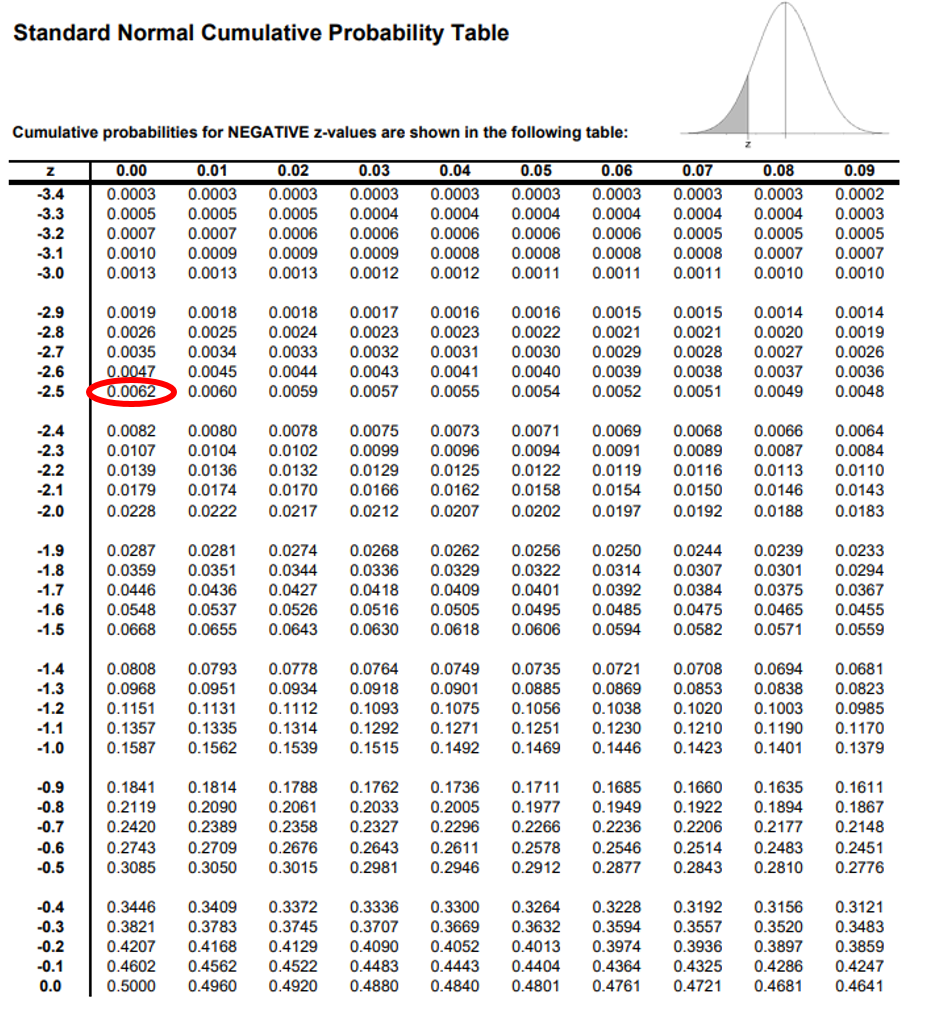
\includegraphics{images/ztable.png}\\

The CDF's corresponding z-value is 0.0062. This means the probability of
a box's weight/can being \textless420.75g is 0.62\%. To work out the
expectation of the fine:

\[
\Large
E(\text{Fine}) = 3000 \times 0.0062 = 18.6
\]

Thus for A:

\[
\Large
E(\text{Fine})=£18.60\text{/box}
\]\\
\strut \\
\strut \\
\strut \\
\strut \\

\subsubsection{B:}\label{b}

I need to calculate the CDF \(F(x) = P(X ≤ 421.8)\). I will use the same
logic as before and calculate the z-value before consulting the table.
This time, \(X = 421.8\) and \(n = 25\) which means that to calculate
the z-value: \[
\Large
\sigma_{\text{sample}} = \frac{\sigma}{\sqrt{n}} = \frac{21}{\sqrt{25}} = 4.2
\]

This higher \(\sigma\) compared to the previous question is to be
expected given the smaller sample size. Thus:

\[
\Large
Z = \frac{421.8 - 426}{4.2} = -1
\]\\

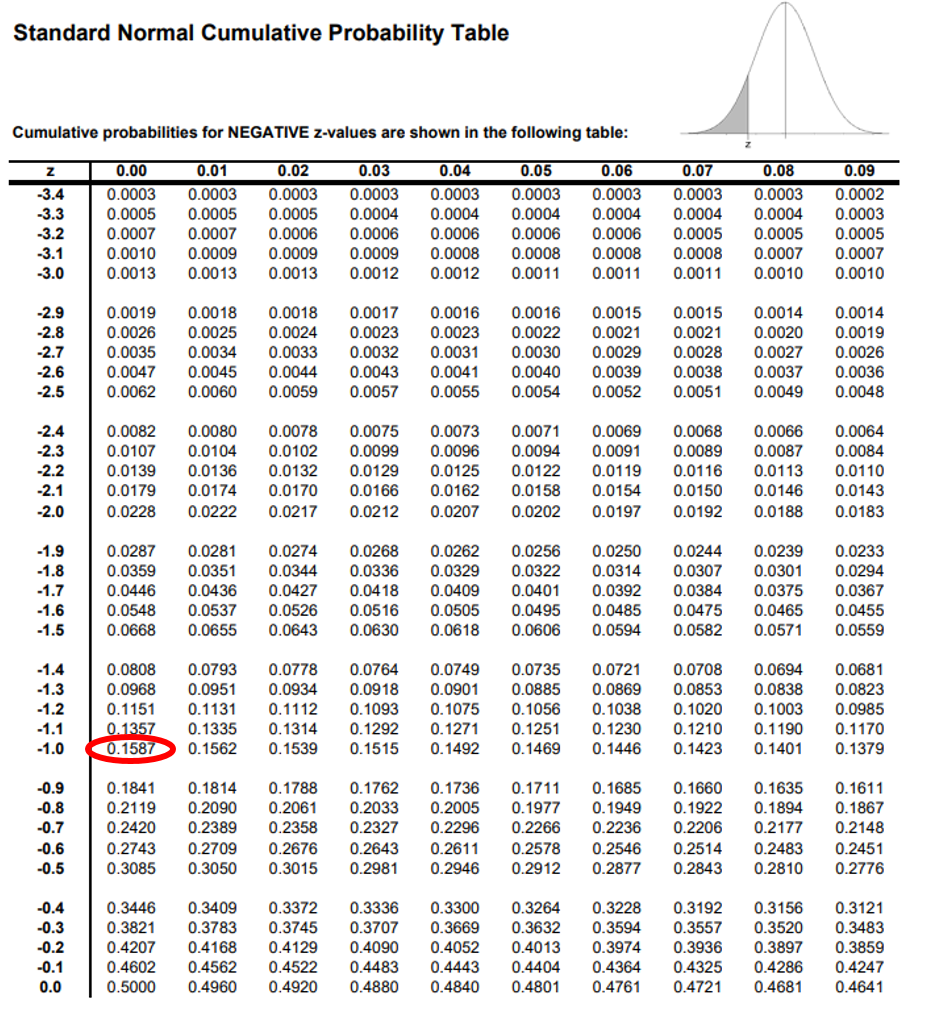
\includegraphics{images/ztableb.png}\\

The CDF's corresponding z-value is 0.1587. This means the probability of
a box's weight/can being \textless421.8g is 15.87\%. To work out the
expectation of the fine:

\[
\Large
E(\text{Fine}) = 120 \times 0.1587 = 19.044
\]

Thus for B:

\[
\Large
E(\text{Fine})=£19.04\text{/box}
\]\\
\strut \\
\strut \\
\strut \\
\strut \\

\subsubsection{C:}\label{c}

The probability that X \textgreater{} 426 is equivalent to
\(1- P(X ≤ 426)\). I could do this again and consult the z-table but
this is unnecessary. 426 is the mean and normally distributed so there
is a 0.5 chance that a randomly sampled can will weigh more and 0.5 that
it will weigh less. Note: this takes into account the fact that a PDF of
a given continuous variable (in this case 426.0g) = 0.

Here, each sampling event is either success \((X > 426)\) or failure
\((X ≤ 426)\) where n could take any number. This is characteristic of
the geometric formula. As discussed, the finite geometric series is:

\[
\Large 
\sum_{n=0}^{\infty}r^n=\frac{1}{1-r} 
\]\\

Since the probability of success = 0.5:

\[
\Large
\sum_{n=0}^{\infty}r^n=\frac{1}{1-0.5}  = 2
\]

As expected, it takes two trials until a success is expected. In turn:

\[
\Large
E(n) = 2
\]

N itself however will have its own distribution which must be considered
before plugging into the fine equation. The variance of n can be
calculated using the variance formula for geometric distributions:

\[
\Large
Var(n) = \frac{1-p}{p^2}
\]

Thus,

\[
\Large
Var(n) = \frac{1-0.5}{0.5^2}= 2
\]\\

To calculate the expectation of the fine I need to use the formula,

\[
\Large
E(n^2) = \text{Var}(n) + (E(n))^2
\]

I have the variance and expected no. samples until success but i also
need the expectation of n\^{}2 because \(n(n−1)=n^2−n\). Therefore to
calculate the expectation of \(n^2\):

\[
\Large
E(n)^2 = 4 + 2^2 = 6
\]

Now I can calculate the E(n(n-1)):

\[
\Large
E(n(n-1))=  E(n^2) - E(n) = 6-2 = 4
\]

Now I have \(E(n(n-1))\), I can plug it into the equation:

\[
\Large
E(\text{Fine}) = 5\times{}E(n(n-1))=  5 \times 4 = 20
\]

In conclusion:

\[
\Large
E(\text{Fine}) =  £20/\text{box}
\]

\hfill\break
\hfill\break
\hfill\break
\hfill\break

\subsection{Question 4a}\label{question-4a}

\paragraph{Introducing the random
variables:}\label{introducing-the-random-variables}

Individually, \(X_i^{(1)}\) and \(X_i^{(2)}\) random variables follow
Bernoulli distributions because its success/failure (outcomes sum to 1),
each trial is independent and \(n\) is 1.

\[
\Large
X_i^{(1)} = \left\{
\begin{array}{ll}
1, & \text{if B supporter number } i \text{ still supports B at the end of day 1}, \\
0, & \text{if B supporter number } i \text{ changes to an M supporter at the end of day 1}.
\end{array}
\right.
\]

For \(i =1...,175\) this is equivalent to:

\[
\Large
X_i^{(1)} = \left\{
\begin{array}{ll}
k= 1, \text{ }p = 1- 0.004 = 0.996 \\
k= 0, \text{ }1-p = 1- 0.996 = 0.004
\end{array}
\right.
\]

In summary, each random variables can be denoted as
\(X_i^{(1)} \sim \text{Bernoulli}(1,p)\text{ for } i = 1...,175\).

\hfill\break

For \(X^{(2)}\):

\[
\Large
X_i^{(2)} = \left\{
\begin{array}{ll}
1, & \text{if M supporter number } i \text{ changes to a B supporter at the end of day 1}, \\
0, & \text{if M supporter number } i \text{ still supports M at the end of day 1}.
\end{array}
\right.
\]

for \(i =1...,186\), this is equivalent to:

\[
\Large
X_i^{(2)} = \left\{
\begin{array}{ll}
k=1, \text{ }p = 0.005 \\
k=0, \text{ }1-p = 1- 0.005 = 0.996
\end{array}
\right.
\]

Again, each random variable trial can be denoted as
\(X_i^{(2)} \sim \text{Bernoulli}(1,p) \text{ for } i = 1...,186\).\\

\hfill\break
\hfill\break

\paragraph{Expressing the number of B supporters at the end of the first
day:}\label{expressing-the-number-of-b-supporters-at-the-end-of-the-first-day}

Every trial is independent and peoples allegiance has no bearing on
other people. Crucially, distinct Bernoulli trials are repeated; not the
same Bernoulli trial. This is because every \(X\) is unique within a
given day i.e.~unique random variables (prospective voters). This
precludes the use of the Binomial distribution characteristics; using
binomial formulas would imply that the Bernoulli trials are repeated on
single person n within a single day. This is not the case.

The number of B supporters at the end of day 1 will be the B's Initial
supporters - those that switch allegiance to support M + those that
switch allegiance to support B:

\[
\text{B supporters after 1 day} =\text{B  supporters at the start of day} - \text{Supporters who switch to M} + \text{Supporters who switch to B}
\]\\
\strut \\

Here I will denote `B supporters at the start of the day' as `B' and M
supporters at the start of the day as `M' which are both integers. Using
the introduced Random distributions this gives:

\[
\Large
\text{B supporters after 1 day} = B -  (B-\sum_{i=1}^{B} X_i^{(1)}) +  \sum_{i=1}^{M}X_i^{(2)}
\]\\

The \((B-\sum_{i=1}^{B} X_i^{(1)})\) is included as it is all the failed
trials for \(X_i^{(1)}\) minus the number of B supporters who switch.
The sum symbol is sufficient here because if a trial ends in success,the
output is 1. This represents a person so the sum of these will equate to
the number of successes. Therefore, probabilities such as \('p'\) and
\('p-1'\) do not need to be expressed in the equation above.\\
\strut \\
\strut \\

\paragraph{Expected number of B supporters at the end of the first
day:}\label{expected-number-of-b-supporters-at-the-end-of-the-first-day}

Using the formula, I can calculate the E(B supporters after one day). I
must first calculate the sum of the expected occurrences in the two
\(X_i^{(1)}\) and \(X_i^{(2)}\) terms.

I can use the properties of the expectation to calculate these. Because
I'm not working with a binomial distribution I will not use its
expectation formula. Instead, I will use the expectation formula for the
Bernoulli: E(X) = p.~Therefore p can be multiplied for the number of
Bernoulli trials in each term:

expectations For
\(E(\sum_{i=1}^{175} X_i^{(1)}) = 175 \times  0.996 = 174.3 = 174\)

For \(E(\sum_{i=1}^{186}X_i^{(2)}) = 186 \times 0.005 = 0.93 = 1\)\\

I have rounded these numbers to the nearest integer as people can cast
either 1 or 0 votes.

Our terms are:

\begin{itemize}
\item
  \(B = 175\)\\
\item
  \(M = 186\)\\
\item
  \(E(\sum_{i=1}^{175} X_i^{(1)}) = 174\)\\
\item
  \(E(\sum_{i=1}^{186}X_i^{(2)})  = 1\)\\
  \strut \\
\end{itemize}

Substituting these values gives:\\

\[
\Large
\text{B supporters after 1 day} = 175 -  (175-174) +  1 
\]\\

Thus:\\
\[
\Large
\text{B supporters after 1 day} = 175
\]\\
\strut \\
\strut \\
\strut \\
\strut \\

\subsection{Question 4b}\label{question-4b}

\paragraph{Number of M supporters at end of first
day:}\label{number-of-m-supporters-at-end-of-first-day}

\[
\text{M supporters after 1 day} =\text{M  supporters at the start of day} + \text{Supporters who switch to M} - \text{Supporters who switch to B}
\]\\

Therefore:\\
\[
\Large
\text{M supporters after 1 day} = M +  (B-\sum_{i=1}^{B} X_i^{(1)}) -  \sum_{i=1}^{M}X_i^{(2)}
\]\\

Substituting the same values from Question 4a gives:\\

\[
\Large
\text{M supporters after 1 day} = 186 +  (175-174) - 1 
\]\\

Thus:\\
\[
\Large
\text{M supporters after 1 day} = 186
\]\\
\strut \\
\strut \\
\strut \\
\strut \\

\subsection{Question 4c}\label{question-4c}

\begin{Shaded}
\begin{Highlighting}[]
\CommentTok{\# Creating the loops for one day first:}

\CommentTok{\# For the X1 outcomes {-}{-}{-}{-}}

\NormalTok{X1 }\OtherTok{\textless{}{-}} \DecValTok{175}  \CommentTok{\# This will become no. permutations for X1}
\NormalTok{X1\_trials }\OtherTok{\textless{}{-}} \FunctionTok{numeric}\NormalTok{(}\DecValTok{175}\NormalTok{)  }\CommentTok{\# Where outcomes of each Bernoulli trial will be stored}
\NormalTok{X1\_probs }\OtherTok{\textless{}{-}} \FunctionTok{c}\NormalTok{(}\FloatTok{0.996}\NormalTok{, }\FloatTok{0.004}\NormalTok{)  }\CommentTok{\# The two probabilities for each X2 trial}
\NormalTok{results }\OtherTok{\textless{}{-}} \FunctionTok{c}\NormalTok{(}\DecValTok{1}\NormalTok{, }\DecValTok{0}\NormalTok{) }\CommentTok{\# The corresponding outputs for the probabilities above }
\NormalTok{no.\_X1\_successes }\OtherTok{\textless{}{-}} \DecValTok{0}  \CommentTok{\# Initial number of successes (Will grow with loops)}


\ControlFlowTok{for}\NormalTok{(i }\ControlFlowTok{in} \DecValTok{1}\SpecialCharTok{:}\NormalTok{X1)\{  }\CommentTok{\# Sampling everyone}
\NormalTok{  X1\_trials[i] }\OtherTok{\textless{}{-}} \FunctionTok{sample}\NormalTok{(results, }
                      \AttributeTok{size =} \DecValTok{1}\NormalTok{, }\CommentTok{\# 1 Bernoulli per person}
                      \AttributeTok{replace =}\NormalTok{ F,  }\CommentTok{\# Only one decision per person (all people must be sampled)}
                      \AttributeTok{prob =}\NormalTok{ X1\_probs)  }\CommentTok{\# Pre{-}specified probabilities}
  \ControlFlowTok{if}\NormalTok{ (X1\_trials[i] }\SpecialCharTok{==} \DecValTok{1}\NormalTok{) \{  }\CommentTok{\# \textquotesingle{}If current trial is a success...\textquotesingle{}}
\NormalTok{    no.\_X1\_successes }\OtherTok{\textless{}{-}}\NormalTok{ no.\_X1\_successes }\SpecialCharTok{+} \DecValTok{1}  \CommentTok{\# \textquotesingle{}...Increase the number of success by 1}
\NormalTok{  \}}
\NormalTok{\}}

\FunctionTok{print}\NormalTok{(no.\_X1\_successes)}




\CommentTok{\# For X2 outcomes {-}{-}{-}{-}}

\NormalTok{X2 }\OtherTok{\textless{}{-}} \DecValTok{186}  \CommentTok{\# This will become no. permutations for X1}
\NormalTok{X2\_trials }\OtherTok{\textless{}{-}} \FunctionTok{numeric}\NormalTok{(}\DecValTok{186}\NormalTok{)  }\CommentTok{\# Where outcomes of each Bernoulli trial will be stored}
\NormalTok{X2\_probs }\OtherTok{\textless{}{-}} \FunctionTok{c}\NormalTok{(}\FloatTok{0.005}\NormalTok{, }\FloatTok{0.996}\NormalTok{)  }\CommentTok{\# The two probabilities for each X2 trial}
\NormalTok{results }\OtherTok{\textless{}{-}} \FunctionTok{c}\NormalTok{(}\DecValTok{1}\NormalTok{, }\DecValTok{0}\NormalTok{) }\CommentTok{\# The corresponding outputs for the probabilities above }
\NormalTok{no.\_X2\_successes }\OtherTok{\textless{}{-}} \DecValTok{0}  \CommentTok{\# Initial number of successes (Will grow with loops)}


\ControlFlowTok{for}\NormalTok{(i }\ControlFlowTok{in} \DecValTok{1}\SpecialCharTok{:}\NormalTok{X2)\{  }\CommentTok{\# Sampling everyone}
\NormalTok{  X2\_trials[i] }\OtherTok{\textless{}{-}} \FunctionTok{sample}\NormalTok{(results, }
                      \AttributeTok{size =} \DecValTok{1}\NormalTok{, }\CommentTok{\# 1 Bernoulli per person}
                      \AttributeTok{replace =}\NormalTok{ F,  }\CommentTok{\# Only one decision per person (all people must be sampled)}
                      \AttributeTok{prob =}\NormalTok{ X2\_probs)  }\CommentTok{\# Pre{-}specificed probabilities}
  \ControlFlowTok{if}\NormalTok{ (X2\_trials[i] }\SpecialCharTok{==} \DecValTok{1}\NormalTok{) \{  }\CommentTok{\# \textquotesingle{}If current trial is a success...\textquotesingle{}}
\NormalTok{    no.\_X2\_successes }\OtherTok{\textless{}{-}}\NormalTok{ no.\_X2\_successes }\SpecialCharTok{+} \DecValTok{1}  \CommentTok{\# \textquotesingle{}...Increase the number of success by 1}
\NormalTok{  \}}
\NormalTok{\}}


\FunctionTok{print}\NormalTok{(no.\_X2\_successes)}

\NormalTok{No.\_B }\OtherTok{\textless{}{-}}\NormalTok{ X1 }\SpecialCharTok{{-}}\NormalTok{ (X1 }\SpecialCharTok{{-}}\NormalTok{ no.\_X1\_successes) }\SpecialCharTok{+}\NormalTok{ no.\_X2\_successes  }\CommentTok{\# No. B supporters after Day 1}
\NormalTok{No.\_M }\OtherTok{\textless{}{-}} \DecValTok{361} \SpecialCharTok{{-}}\NormalTok{ No.\_B  }\CommentTok{\# No. M supporters after Day 1}









\CommentTok{\# Now I need to have this iterated 14 times but have \textquotesingle{}No.\_B\textquotesingle{} and \textquotesingle{}No.\_M\textquotesingle{} values}
\CommentTok{\# assigned to the \textquotesingle{}X1\textquotesingle{} and \textquotesingle{}X1\_trials\textquotesingle{} and \textquotesingle{}X2\textquotesingle{} and \textquotesingle{}X2\_trials\textquotesingle{} respectively }

\CommentTok{\# For the 14 days:}
\NormalTok{no.\_iterations }\OtherTok{\textless{}{-}} \DecValTok{14}  \CommentTok{\# No. days }


\NormalTok{X1 }\OtherTok{\textless{}{-}} \DecValTok{175}  \CommentTok{\# This will become no. permutations for X1}
\NormalTok{X1\_trials }\OtherTok{\textless{}{-}} \FunctionTok{numeric}\NormalTok{(}\DecValTok{175}\NormalTok{)  }\CommentTok{\# Where outcomes of each Bernoulli trial will be stored}
\NormalTok{no.\_X1\_successes }\OtherTok{\textless{}{-}} \DecValTok{0}  \CommentTok{\# Initial number of successes (Will grow with loops)}

\NormalTok{X2 }\OtherTok{\textless{}{-}} \DecValTok{186}  \CommentTok{\# This will become no. permutations for X1}
\NormalTok{X2\_trials }\OtherTok{\textless{}{-}} \FunctionTok{numeric}\NormalTok{(}\DecValTok{186}\NormalTok{)  }\CommentTok{\# Where outcomes of each Bernoulli trial will be stored}
\NormalTok{no.\_X2\_successes }\OtherTok{\textless{}{-}} \DecValTok{0}  \CommentTok{\# Initial number of successes (Will grow with loops)}



\ControlFlowTok{for}\NormalTok{ (day }\ControlFlowTok{in} \DecValTok{1}\SpecialCharTok{:}\NormalTok{no.\_iterations) \{ }\CommentTok{\# Loop for each day (n = 14)}
\NormalTok{  X1\_trials }\OtherTok{\textless{}{-}} \FunctionTok{numeric}\NormalTok{(X1)  }\CommentTok{\# Store outcomes for X1 trials}
\NormalTok{  no.\_X1\_successes }\OtherTok{\textless{}{-}} \DecValTok{0}  \CommentTok{\# Reset success count for X1}
  
  \ControlFlowTok{for}\NormalTok{ (i }\ControlFlowTok{in} \DecValTok{1}\SpecialCharTok{:}\NormalTok{X1) \{}
\NormalTok{    X1\_trials[i] }\OtherTok{\textless{}{-}} \FunctionTok{sample}\NormalTok{(results, }\AttributeTok{size =} \DecValTok{1}\NormalTok{, }\AttributeTok{replace =} \ConstantTok{FALSE}\NormalTok{, }\AttributeTok{prob =}\NormalTok{ X1\_probs)}
    \ControlFlowTok{if}\NormalTok{ (X1\_trials[i] }\SpecialCharTok{==} \DecValTok{1}\NormalTok{) \{}
\NormalTok{      no.\_X1\_successes }\OtherTok{\textless{}{-}}\NormalTok{ no.\_X1\_successes }\SpecialCharTok{+} \DecValTok{1}
\NormalTok{    \}}
\NormalTok{  \}}
  
  \CommentTok{\# For X2 outcomes}
\NormalTok{  X2\_trials }\OtherTok{\textless{}{-}} \FunctionTok{numeric}\NormalTok{(X2)  }\CommentTok{\# Store outcomes for X2 trials}
\NormalTok{  no.\_X2\_successes }\OtherTok{\textless{}{-}} \DecValTok{0}  \CommentTok{\# Reset success count for X2}
  
  \ControlFlowTok{for}\NormalTok{ (i }\ControlFlowTok{in} \DecValTok{1}\SpecialCharTok{:}\NormalTok{X2) \{}
\NormalTok{    X2\_trials[i] }\OtherTok{\textless{}{-}} \FunctionTok{sample}\NormalTok{(results, }\AttributeTok{size =} \DecValTok{1}\NormalTok{, }\AttributeTok{replace =} \ConstantTok{FALSE}\NormalTok{, }\AttributeTok{prob =}\NormalTok{ X2\_probs)}
    \ControlFlowTok{if}\NormalTok{ (X2\_trials[i] }\SpecialCharTok{==} \DecValTok{1}\NormalTok{) \{}
\NormalTok{      no.\_X2\_successes }\OtherTok{\textless{}{-}}\NormalTok{ no.\_X2\_successes }\SpecialCharTok{+} \DecValTok{1}
\NormalTok{    \}}
\NormalTok{  \}}
  
  \CommentTok{\# Calculate No.\_B and No.\_M}
\NormalTok{  No.\_B }\OtherTok{\textless{}{-}}\NormalTok{ X1 }\SpecialCharTok{{-}}\NormalTok{ (X1 }\SpecialCharTok{{-}}\NormalTok{ no.\_X1\_successes) }\SpecialCharTok{+}\NormalTok{ no.\_X2\_successes}
\NormalTok{  No.\_M }\OtherTok{\textless{}{-}} \DecValTok{361} \SpecialCharTok{{-}}\NormalTok{ No.\_B}
  
  \CommentTok{\# Update X1 and X2 for the next iteration}
\NormalTok{  X1 }\OtherTok{\textless{}{-}}\NormalTok{ No.\_B}
\NormalTok{  X2 }\OtherTok{\textless{}{-}}\NormalTok{ No.\_M}
\NormalTok{\}}

\FunctionTok{print}\NormalTok{(X1)  }\CommentTok{\# No. B supporters after 14 days}
\FunctionTok{print}\NormalTok{(X2)  }\CommentTok{\# No M supporters after 14 days}














\CommentTok{\# Now to work out the probability that No.\_B \textgreater{} No.\_M, I will nest one more loop}
\CommentTok{\# I will repeat the 14 days experiment thousands of times and }
\CommentTok{\# calculate what proportion of the outputs have No.\_B \textgreater{} No.\_M}


\CommentTok{\# Final loop iterations {-}{-}{-}{-}}
\NormalTok{simulations }\OtherTok{\textless{}{-}} \DecValTok{10000}  \CommentTok{\# This sample size willallow the true probability to be inferred confidently}
\NormalTok{B\_more\_than\_M }\OtherTok{\textless{}{-}} \DecValTok{0}  \CommentTok{\# Intial No. where B \textgreater{} M}


\NormalTok{X1 }\OtherTok{\textless{}{-}} \DecValTok{175}  \CommentTok{\# This will become no. permutations for X1}
\NormalTok{X1\_trials }\OtherTok{\textless{}{-}} \FunctionTok{numeric}\NormalTok{(}\DecValTok{175}\NormalTok{)  }\CommentTok{\# Where outcomes of each Bernoulli trial will be stored}
\NormalTok{no.\_X1\_successes }\OtherTok{\textless{}{-}} \DecValTok{0}  \CommentTok{\# Initial number of successes (Will grow with loops)}

\NormalTok{X2 }\OtherTok{\textless{}{-}} \DecValTok{186}  \CommentTok{\# This will become no. permutations for X1}
\NormalTok{X2\_trials }\OtherTok{\textless{}{-}} \FunctionTok{numeric}\NormalTok{(}\DecValTok{186}\NormalTok{)  }\CommentTok{\# Where outcomes of each Bernoulli trial will be stored}
\NormalTok{no.\_X2\_successes }\OtherTok{\textless{}{-}} \DecValTok{0}  \CommentTok{\# Initial number of successes (Will grow with loops)}



\CommentTok{\# Run the simulation 10000 times}
\ControlFlowTok{for}\NormalTok{ (sim }\ControlFlowTok{in} \DecValTok{1}\SpecialCharTok{:}\NormalTok{simulations) \{}
  
  \CommentTok{\# Run the 14{-}iteration loop}
  \ControlFlowTok{for}\NormalTok{ (day }\ControlFlowTok{in} \DecValTok{1}\SpecialCharTok{:}\NormalTok{no.\_iterations) \{}
    \CommentTok{\# For X1 outcomes}
\NormalTok{    X1\_trials }\OtherTok{\textless{}{-}} \FunctionTok{numeric}\NormalTok{(X1)}
\NormalTok{    no.\_X1\_successes }\OtherTok{\textless{}{-}} \DecValTok{0}
    
    \ControlFlowTok{for}\NormalTok{ (i }\ControlFlowTok{in} \DecValTok{1}\SpecialCharTok{:}\NormalTok{X1) \{}
\NormalTok{      X1\_trials[i] }\OtherTok{\textless{}{-}} \FunctionTok{sample}\NormalTok{(results, }\AttributeTok{size =} \DecValTok{1}\NormalTok{, }\AttributeTok{replace =} \ConstantTok{FALSE}\NormalTok{, }\AttributeTok{prob =}\NormalTok{ X1\_probs)}
      \ControlFlowTok{if}\NormalTok{ (X1\_trials[i] }\SpecialCharTok{==} \DecValTok{1}\NormalTok{) \{}
\NormalTok{        no.\_X1\_successes }\OtherTok{\textless{}{-}}\NormalTok{ no.\_X1\_successes }\SpecialCharTok{+} \DecValTok{1}
\NormalTok{      \}}
\NormalTok{    \}}
    
    \CommentTok{\# For X2 outcomes}
\NormalTok{    X2\_trials }\OtherTok{\textless{}{-}} \FunctionTok{numeric}\NormalTok{(X2)}
\NormalTok{    no.\_X2\_successes }\OtherTok{\textless{}{-}} \DecValTok{0}
    
    \ControlFlowTok{for}\NormalTok{ (i }\ControlFlowTok{in} \DecValTok{1}\SpecialCharTok{:}\NormalTok{X2) \{}
\NormalTok{      X2\_trials[i] }\OtherTok{\textless{}{-}} \FunctionTok{sample}\NormalTok{(results, }\AttributeTok{size =} \DecValTok{1}\NormalTok{, }\AttributeTok{replace =} \ConstantTok{FALSE}\NormalTok{, }\AttributeTok{prob =}\NormalTok{ X2\_probs)}
      \ControlFlowTok{if}\NormalTok{ (X2\_trials[i] }\SpecialCharTok{==} \DecValTok{1}\NormalTok{) \{}
\NormalTok{        no.\_X2\_successes }\OtherTok{\textless{}{-}}\NormalTok{ no.\_X2\_successes }\SpecialCharTok{+} \DecValTok{1}
\NormalTok{      \}}
\NormalTok{    \}}
    
    \CommentTok{\# Calculate No.\_B and No.\_M}
\NormalTok{    No.\_B }\OtherTok{\textless{}{-}}\NormalTok{ X1 }\SpecialCharTok{{-}}\NormalTok{ (X1 }\SpecialCharTok{{-}}\NormalTok{ no.\_X1\_successes) }\SpecialCharTok{+}\NormalTok{ no.\_X2\_successes}
\NormalTok{    No.\_M }\OtherTok{\textless{}{-}} \DecValTok{361} \SpecialCharTok{{-}}\NormalTok{ No.\_B}
    
    \CommentTok{\# Update X1 and X2 for the next iteration}
\NormalTok{    X1 }\OtherTok{\textless{}{-}}\NormalTok{ No.\_B}
\NormalTok{    X2 }\OtherTok{\textless{}{-}}\NormalTok{ No.\_M}
\NormalTok{  \}}
  
  \CommentTok{\# Check if No.\_B \textgreater{} No.\_M in the final result and count it}
  \ControlFlowTok{if}\NormalTok{ (No.\_B }\SpecialCharTok{\textgreater{}}\NormalTok{ No.\_M) \{}
\NormalTok{    B\_more\_than\_M }\OtherTok{\textless{}{-}}\NormalTok{ B\_more\_than\_M }\SpecialCharTok{+} \DecValTok{1}
\NormalTok{  \}}
\NormalTok{\}}

\NormalTok{answer }\OtherTok{\textless{}{-}}\NormalTok{ B\_more\_than\_M}\SpecialCharTok{/} \DecValTok{10000}  \CommentTok{\# Average number of times B has the majority}

\FunctionTok{print}\NormalTok{(answer)  }\CommentTok{\# = 0.098}
\end{Highlighting}
\end{Shaded}

\subsection{Question 4d}\label{question-4d}

\begin{Shaded}
\begin{Highlighting}[]
\CommentTok{\# Repeat but change no. iterations to 60}
\NormalTok{no.\_iterations\_60 }\OtherTok{\textless{}{-}} \DecValTok{60}  \CommentTok{\# No. days }

\CommentTok{\# Final loop iterations {-}{-}{-}{-}}
\NormalTok{simulations }\OtherTok{\textless{}{-}} \DecValTok{10000}  \CommentTok{\# This sample size willallow the true probability to be inferred confidently}
\NormalTok{B\_more\_than\_M }\OtherTok{\textless{}{-}} \DecValTok{0}  \CommentTok{\# Intial No. where B \textgreater{} M}


\NormalTok{X1 }\OtherTok{\textless{}{-}} \DecValTok{175}  \CommentTok{\# This will become no. permutations for X1}
\NormalTok{X1\_trials }\OtherTok{\textless{}{-}} \FunctionTok{numeric}\NormalTok{(}\DecValTok{175}\NormalTok{)  }\CommentTok{\# Where outcomes of each Bernoulli trial will be stored}
\NormalTok{no.\_X1\_successes }\OtherTok{\textless{}{-}} \DecValTok{0}  \CommentTok{\# Initial number of successes (Will grow with loops)}

\NormalTok{X2 }\OtherTok{\textless{}{-}} \DecValTok{186}  \CommentTok{\# This will become no. permutations for X1}
\NormalTok{X2\_trials }\OtherTok{\textless{}{-}} \FunctionTok{numeric}\NormalTok{(}\DecValTok{186}\NormalTok{)  }\CommentTok{\# Where outcomes of each Bernoulli trial will be stored}
\NormalTok{no.\_X2\_successes }\OtherTok{\textless{}{-}} \DecValTok{0}  \CommentTok{\# Initial number of successes (Will grow with loops)}



\CommentTok{\# Run the simulation 10000 times}
\ControlFlowTok{for}\NormalTok{ (sim }\ControlFlowTok{in} \DecValTok{1}\SpecialCharTok{:}\NormalTok{simulations) \{}
  
  \CommentTok{\# Run the 14{-}iteration loop}
  \ControlFlowTok{for}\NormalTok{ (day }\ControlFlowTok{in} \DecValTok{1}\SpecialCharTok{:}\NormalTok{no.\_iterations\_60) \{}
    \CommentTok{\# For X1 outcomes}
\NormalTok{    X1\_trials }\OtherTok{\textless{}{-}} \FunctionTok{numeric}\NormalTok{(X1)}
\NormalTok{    no.\_X1\_successes }\OtherTok{\textless{}{-}} \DecValTok{0}
    
    \ControlFlowTok{for}\NormalTok{ (i }\ControlFlowTok{in} \DecValTok{1}\SpecialCharTok{:}\NormalTok{X1) \{}
\NormalTok{      X1\_trials[i] }\OtherTok{\textless{}{-}} \FunctionTok{sample}\NormalTok{(results, }\AttributeTok{size =} \DecValTok{1}\NormalTok{, }\AttributeTok{replace =} \ConstantTok{FALSE}\NormalTok{, }\AttributeTok{prob =}\NormalTok{ X1\_probs)}
      \ControlFlowTok{if}\NormalTok{ (X1\_trials[i] }\SpecialCharTok{==} \DecValTok{1}\NormalTok{) \{}
\NormalTok{        no.\_X1\_successes }\OtherTok{\textless{}{-}}\NormalTok{ no.\_X1\_successes }\SpecialCharTok{+} \DecValTok{1}
\NormalTok{      \}}
\NormalTok{    \}}
    
    \CommentTok{\# For X2 outcomes}
\NormalTok{    X2\_trials }\OtherTok{\textless{}{-}} \FunctionTok{numeric}\NormalTok{(X2)}
\NormalTok{    no.\_X2\_successes }\OtherTok{\textless{}{-}} \DecValTok{0}
    
    \ControlFlowTok{for}\NormalTok{ (i }\ControlFlowTok{in} \DecValTok{1}\SpecialCharTok{:}\NormalTok{X2) \{}
\NormalTok{      X2\_trials[i] }\OtherTok{\textless{}{-}} \FunctionTok{sample}\NormalTok{(results, }\AttributeTok{size =} \DecValTok{1}\NormalTok{, }\AttributeTok{replace =} \ConstantTok{FALSE}\NormalTok{, }\AttributeTok{prob =}\NormalTok{ X2\_probs)}
      \ControlFlowTok{if}\NormalTok{ (X2\_trials[i] }\SpecialCharTok{==} \DecValTok{1}\NormalTok{) \{}
\NormalTok{        no.\_X2\_successes }\OtherTok{\textless{}{-}}\NormalTok{ no.\_X2\_successes }\SpecialCharTok{+} \DecValTok{1}
\NormalTok{      \}}
\NormalTok{    \}}
    
    \CommentTok{\# Calculate No.\_B and No.\_M}
\NormalTok{    No.\_B }\OtherTok{\textless{}{-}}\NormalTok{ X1 }\SpecialCharTok{{-}}\NormalTok{ (X1 }\SpecialCharTok{{-}}\NormalTok{ no.\_X1\_successes) }\SpecialCharTok{+}\NormalTok{ no.\_X2\_successes}
\NormalTok{    No.\_M }\OtherTok{\textless{}{-}} \DecValTok{361} \SpecialCharTok{{-}}\NormalTok{ No.\_B}
    
    \CommentTok{\# Update X1 and X2 for the next iteration}
\NormalTok{    X1 }\OtherTok{\textless{}{-}}\NormalTok{ No.\_B}
\NormalTok{    X2 }\OtherTok{\textless{}{-}}\NormalTok{ No.\_M}
\NormalTok{  \}}
  
  \CommentTok{\# Check if No.\_B \textgreater{} No.\_M in the final result and count it}
  \ControlFlowTok{if}\NormalTok{ (No.\_B }\SpecialCharTok{\textgreater{}}\NormalTok{ No.\_M) \{}
\NormalTok{    B\_more\_than\_M }\OtherTok{\textless{}{-}}\NormalTok{ B\_more\_than\_M }\SpecialCharTok{+} \DecValTok{1}
\NormalTok{  \}}
\NormalTok{\}}

\NormalTok{answer }\OtherTok{\textless{}{-}}\NormalTok{ B\_more\_than\_M}\SpecialCharTok{/} \DecValTok{10000}  \CommentTok{\# Average number of times B has the majority}

\FunctionTok{print}\NormalTok{(answer)  }\CommentTok{\# = 0.981}
\end{Highlighting}
\end{Shaded}

\paragraph{Conclusion}\label{conclusion}

P(B\textgreater M after 60 days) = 0.981 = 98.1\%.

The difference in probability of B winning with the delay is:

\[
\Large
0.981 - 0.098 = 0.883 
\] Therefore the increase in B probability of winning following the
delay is: \[
\Large
= +88.3\text%
\]\\
\strut \\
\strut \\
\strut \\
\strut \\

\subsection{Question 5a}\label{question-5a}

One important feature of the poisson distribution is that lambda (λ)
represents the mean and the sample variance as they should be
approximately equal values. Therefore I can consider both as foundations
for calculating point estimation. To calculate the mean no. strikes I
can do (3sf):\\

\[
\Large
\bar{y}= \frac{\sum_{i=1}^{182}yi} {n} = \frac{60}{182}=0.330
\] For the sample variance (3sf):\\
\strut \\
\[
\Large
s^2 = \frac{1}{n - 1} \sum_{i=1}^{n} y_i = \frac{1}{182-1}\times60 = 0.331 
\]\\
\strut \\

I have proven that there can be 2 estimates for lambda. However, the
mean is regarded as a better foundation for an estimator as it tends to
be more concentrated around the true value of lambda than variance.
Therefore, I will continue with the first lambda estimate.

Now I can scrutinise whether my suggested estimator is bias or not:

\(\hat{\lambda} =  \frac{\sum_{i=1}^{n}yi} {n}  =y ̄\) Bias:
\(\text{Bias}(\lambda)= E(\lambda)- \lambda\)
\(E(\lambda) = E(\frac{\sum_{i=1}^{n}yi} {n}) = \frac{\sum_{i=1}^{n}E(yi)} {n}\)
\(E(yi)= \lambda\)

Therefore: \(E(\lambda) = \frac{n\times \lambda} {n} = \lambda\)\\

In turn:
\(\text{Bias}(\lambda)= E(\lambda)- \lambda = \lambda - \lambda = 0\)

I have proved that the estimator is not bias. Furthermore, the sample
mean is known to be a consistent estimator of lambda. Now I can
calculate the standard error for the estimator.

\paragraph{Standard Error}\label{standard-error}

Standard error = sd of the sample mean:

\[
\Large
se = \frac{\sigma}{\sqrt{n}} = \sqrt{\frac{1}{n}\text{ Var}(X)}
\] As previously calculated, the sample variance = 0.331. Therefore :

\[
\Large
se \text{ (3sf)}= \sqrt{\frac{1}{182}\times 0.331} = 0.0426 
\]\\
\strut \\
\strut \\
\strut \\

\paragraph{Calculating 95\% confidence intervals for
λ}\label{calculating-95-confidence-intervals-for-ux3bb}

While the data does not have a normal distribution, I can apply the
central limit theorem. The sample size is large (n \textgreater{} 30) so
the sample mean will be approximately normal
(\(\bar{y}\text~ N(\lambda,\frac{\lambda}{n})\)). For a poisson
distribution with a large sample size, we can use the following formula
for a approximate confidence interval:

\[
\Large
95\text{% } CI =\left[ \bar{y} - z_{1 - \frac{\alpha}{2}} \frac{\sigma}{\sqrt{n}}, \, \bar{y} + z_{1 - \frac{\alpha}{2}} \frac{\sigma}{\sqrt{n}} \right]
\]\\
\strut \\
\strut \\
In this case \(\alpha\) 0.05 but by consulting the z-table, I know that
\(z_1\) for a 95\% CI is 1.96. Therefore:

\[
\Large
95\text{% } CI =\left[0.330 - 1.96\times 0.0426, \, 0.330 + 1.96 \times 0.0426\right]
\]\\
\[
\Large
95\text{% } CI =\left[0.247 ,\text{ } 0.414\right]
\]\\

\paragraph{Does the confidence interval support the hypothesis at the
5\%-level that λ =
1?}\label{does-the-confidence-interval-support-the-hypothesis-at-the-5-level-that-ux3bb-1}

At the 5\% level, the confidence intervals do not span 1. Therefore the
parameter lambda is estimated to fall within this interval 95\% of the
time. As a result, the intervals do not support the hypothesis at the
5\% level. Additionally, it does span any value ≥ 0.5 so if we were to
round to the nearest integer, this would be 0, not 1.\\
\strut \\
\strut \\
\strut \\
\strut \\

\subsection{5b}\label{b-1}

I want to find the log of the likelihood function for this discrete
random variable. First I will identify the the likelihood of the given
probability mass function. Therefore:\\
\[
\Large
L(y;λ) = L(\frac{ e^{-\lambda}\lambda^y }{(1 - e^{-\lambda})y!}) = 
\prod_{i=1}^{n} \frac{ e^{-\lambda}\lambda^{yi} }{(1 - e^{-\lambda})yi!}
\]\\

Now I can discern the log likelihood (including constants):

\[
\Large
LL(y;\lambda) = ln (L(\lambda))  = 
ln(\prod_{i=1}^{n} \frac{ e^{-\lambda}\lambda^{y_i} }{(1 - e^{-\lambda})y_i!})
= \sum_{i=1}^nln(\frac{ e^{-\lambda}\lambda^{y_i} }{(1 - e^{-\lambda})y_i!})
\]\\

I can use the rule whereby \(ln(ab) = ln(a) + ln(b)\). This also means
that:\\
\[
LL(y;\lambda) = \sum_{i=1}^n
\ln(e^{-\lambda}) + \ln(\lambda y_i) - \ln(1 - e^{-\lambda}) - \ln(y_i!)
\]

Now I will take the sum of the log of each term
(\(\sum_{i=1}^{n} ln(x)\)) and then sum them together using the
\(ln(ab) = ln(a)+ln(b)\). This will allow me to decipher which terms are
constants and rearrange accordingly afterwards.

\[
\sum_{i=1}^{n} ln(e^{-\lambda}) = n\lambda
\]\\
\[
\sum_{i=1}^{n} ln(\lambda^{yi}) = (\sum_{i=1}^ny_i) \times ln (\lambda)
\]\\
\[
\sum_{i=1}^{n} ln(1 - e^{-\lambda}) = n\times ln(1-e^{-\lambda})
\]\\
\[
\sum_{i=1}^{n} ln(yi!) = \sum_{i=1}^{n} ln\text{ }yi!
\]

Given the aforementioned rule whereby ln(ab) = ln(a) + ln(b), this
gives:

\[
\Large
LL(y; \lambda) = -n\lambda +  \sum_{i=1}^n y_i \ln \lambda - n \ln (1 - e^{-\lambda}) - \sum_{i=1}^n ln\text{ }y_i!
\]

To find the maximum likelihood estimate, I can now differentiate this
equation with respect to lambda. I will use partial derivatives because
one term depends on both \(y_i\) and lambda \[
\Large
\frac{d(LL) }{d\lambda}=\frac{d }{d\lambda}(-n\lambda +  \sum_{i=1}^n y_i \ln \lambda - n \ln (1 - e^{-\lambda}) - \sum_{i=1}^n ln\text{ }y_i!)
\]\\

\paragraph{Derivative of each term:}\label{derivative-of-each-term}

Power rule:\\
\strut \\
\[
\frac{d }{d\lambda}(-n\lambda) = -n
\]\\
\strut \\
Chain rule: \(\left( \sum_{i=1}^n y_i \right)\) = constant, f(x) = ln,
g(x) = lambda

\[
\frac{d }{d\lambda}(\left( \sum_{i=1}^n y_i \right) \ln \lambda) = \frac{\sum_{i=1}^n y_i}{\lambda}
\]\\
\strut \\
Chain rule: \(-n\) = constant,
\(f(x) = ln \text{ and } g(x) = 1-e^{-\lambda}\):\\

\[
\frac{d }{d\lambda}(- n \ln (1 - e^{-\lambda})) = -\frac{ne^{-\lambda}}{1-e^{-\lambda}}
\]\\
\strut \\
Derivating a constant (no dependency on lambda):\\

\[
\frac{d }{d\lambda}(\sum_{i=1}^n ln\text{ }y_i!) = 0
\]\\
\strut \\

Therefore:\\
\strut \\
\[
\Large
\frac{d(LL)}{d\lambda} = -n + \frac{\sum_{i=1}^n y_i}{\lambda}-\frac{ne^{-\lambda}}{1-e^{-\lambda}}
\]

Because I'm maximizing the log likelihood model, I now equate this to
0:\\
\strut \\
\[
\Large
\frac{d( LL)}{d\lambda} = -n + \frac{\sum_{i=1}^n y_i}{\lambda}-\frac{ne^{-\lambda}}{1-e^{-\lambda}} =0
\]\\
\strut \\
The lambda value that maximises the likelihood must satisfy this
equation. Now I can rearrange the equation to get the desired form from
the question
(\(\frac{\hat{\lambda}}{1-e^{-\hat{\lambda}}}= \frac{4}{3}\)):\\

\[
\Large
-n + \frac{\sum_{i=1}^n y_i}{\lambda}= \frac{ne^{-\lambda}}{1-e^{-\lambda}} 
\]\\
\strut \\
Now clear the denominators by multiplying by \({1-e^{-\lambda}}\):\\

\[
\Large
-n\lambda(1-e^{-\lambda})  + \sum_{i=1}^n y_i(1-e^{-\lambda}) = ne^{-\lambda}
\]\\

Expanding the brackets gives: \[
\Large
-n\lambda + n\lambda e^{-\lambda} + \sum_{i=1}^n y_i -\sum_{i=1}^ny_ie^{-\lambda} = ne^{-\lambda}
\]\\
\strut \\
Cancel out \(ne^{-\lambda}\):

\[
\Large
-n\lambda + \sum_{i=1}^n y_i -\sum_{i=1}^ny_ie^{-\lambda} = 0
\]\\
\strut \\
This is equivalent to:\\
\strut \\
\[
\Large
\sum_{i=1}^n y_i -n\lambda  = \sum_{i=1}^ny_ie^{-\lambda}
\]\\
\strut \\

Now I can divide by \(\sum_{i=1}^n y_i\):\\
\strut \\
\[
\Large
1-\frac{n\lambda}{ \sum_{i=1}^n y_i }  =  e^{-\lambda}
\]\\
\strut \\
Rearranging gives:\\
\strut \\

\[
\Large
\frac{n\lambda}{ \sum_{i=1}^n y_i }  =  1- e^{-\lambda}
\]\\
\strut \\
Thus:\\
\strut \\
\[
\Large
n\lambda  =  \sum_{i=1}^n y_i  \times \frac{e^\lambda-1}{e^\lambda}
\]\\

Therefore:\\
\[
\Large
\frac{\lambda}{1 - e^{-\lambda}} = \frac{3}{4}
\]\\
\strut \\
\strut \\
\strut \\

\subsection{Question 5c}\label{question-5c}

To plot the
\(-n + \frac{\sum_{i=1}^n y_i}{\lambda}-\frac{ne^{-\lambda}}{1-e^{-\lambda}}\):\\

\begin{Shaded}
\begin{Highlighting}[]
\NormalTok{lambdas }\OtherTok{\textless{}{-}} \FunctionTok{seq}\NormalTok{(}\DecValTok{1}\NormalTok{, }\DecValTok{100}\NormalTok{, }\AttributeTok{length.out =} \DecValTok{100}\NormalTok{) }\CommentTok{\# Creating values from 1{-}100 increasing by intervals of 1 to represent hypothetical lambda values}
\NormalTok{n }\OtherTok{\textless{}{-}} \DecValTok{182}  \CommentTok{\# Using given data from the question (n)}
\NormalTok{sumyi }\OtherTok{\textless{}{-}} \DecValTok{60} \CommentTok{\# Using data from the question (sum of ys)}
\NormalTok{DLL\_values }\OtherTok{\textless{}{-}}  \SpecialCharTok{{-}}\NormalTok{n }\SpecialCharTok{+}\NormalTok{ (sumyi}\SpecialCharTok{/}\NormalTok{lambdas) }\SpecialCharTok{{-}}\NormalTok{ ((n }\SpecialCharTok{*} \FunctionTok{exp}\NormalTok{(}\SpecialCharTok{{-}}\NormalTok{lambdas)) }\SpecialCharTok{/}\NormalTok{ (}\DecValTok{1} \SpecialCharTok{{-}} \FunctionTok{exp}\NormalTok{(}\SpecialCharTok{{-}}\NormalTok{lambdas)))  }\CommentTok{\# Converting the derivative of the LL equation into R}


\NormalTok{plotting\_data }\OtherTok{\textless{}{-}} \FunctionTok{data.frame}\NormalTok{(}\AttributeTok{lambda =}\NormalTok{ lambdas, }\AttributeTok{DLL =}\NormalTok{ DLL\_values)  }\CommentTok{\# Creating a dataframe of the lambdas and DDL vlaues}


\NormalTok{plotting\_data }\SpecialCharTok{\%\textgreater{}\%}  \CommentTok{\# Specifying the dataframe}
  \FunctionTok{ggplot}\NormalTok{(}\FunctionTok{aes}\NormalTok{(}\AttributeTok{x =}\NormalTok{ DLL, }\AttributeTok{y =}\NormalTok{ lambda)) }\SpecialCharTok{+}  \CommentTok{\# Specifying the data}
  \FunctionTok{geom\_point}\NormalTok{() }\SpecialCharTok{+}  \CommentTok{\# Plotting the  data }
  \FunctionTok{geom\_line}\NormalTok{() }\SpecialCharTok{+}  \CommentTok{\# Fitting a line that goes through every points}
  \FunctionTok{theme\_classic}\NormalTok{()  }\CommentTok{\# Removing the background}
\end{Highlighting}
\end{Shaded}

This gives:\\
\strut \\
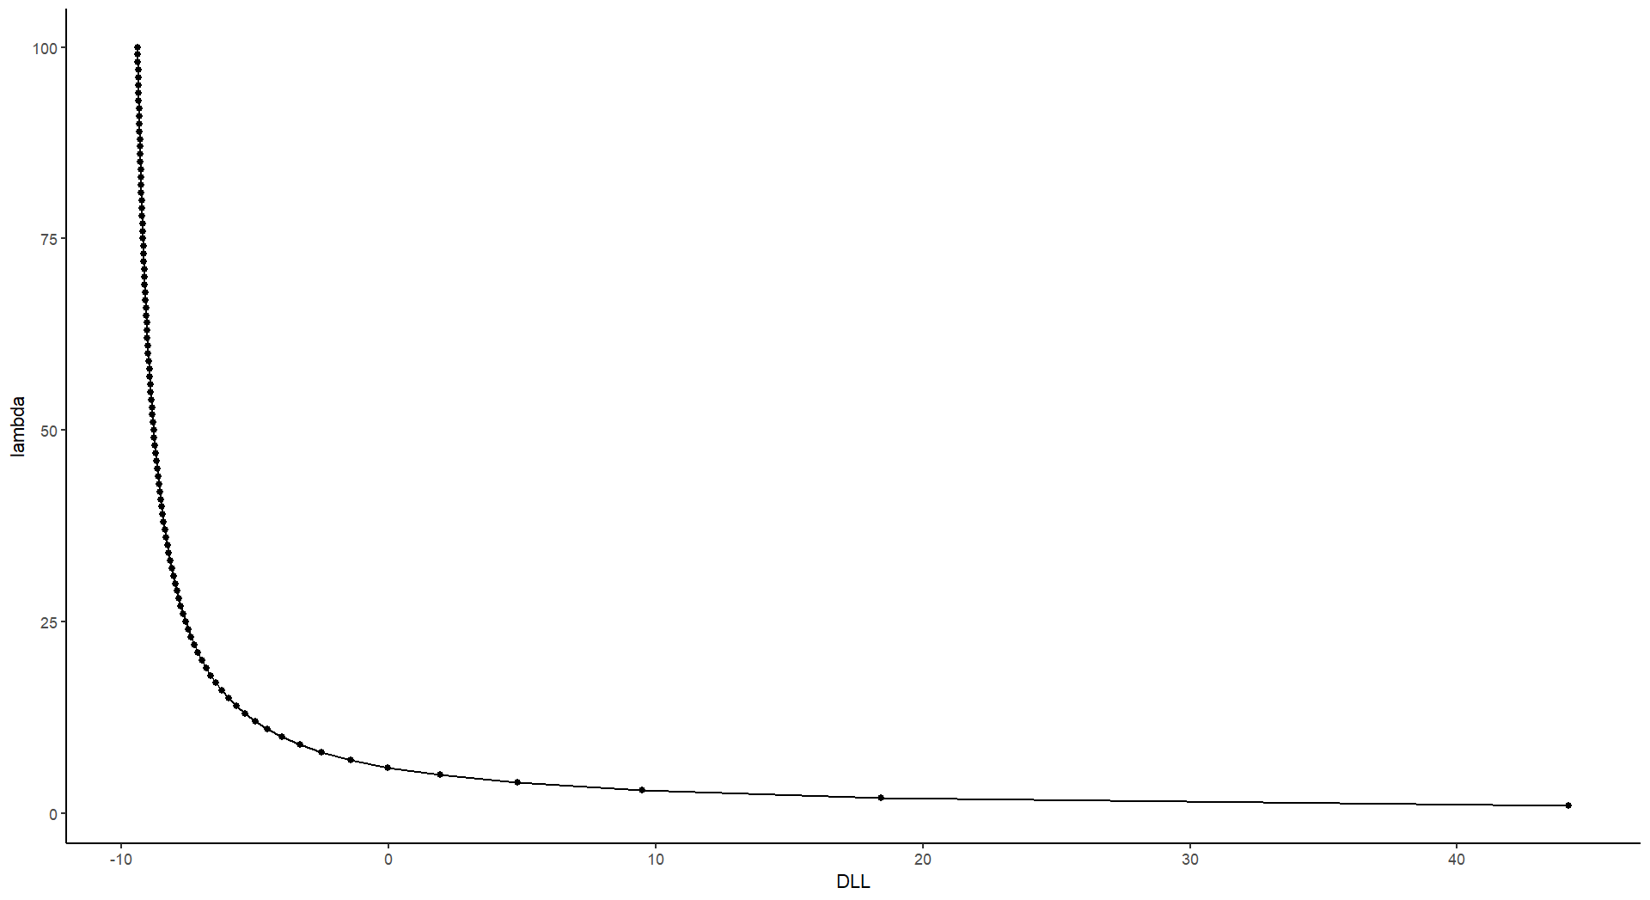
\includegraphics{images/DLL_function.png}\\
\strut \\
I could determine the interval (length 1) where DLL becomes positive
visually (root) but I will use R to be sure:\\
\strut \\

\begin{Shaded}
\begin{Highlighting}[]
\NormalTok{plotting\_data }\SpecialCharTok{\%\textgreater{}\%}  \CommentTok{\# Specifying the dataframe}
  \FunctionTok{ggplot}\NormalTok{(}\FunctionTok{aes}\NormalTok{(}\AttributeTok{x =}\NormalTok{ DLL, }\AttributeTok{y =}\NormalTok{ lambda)) }\SpecialCharTok{+}  \CommentTok{\# Specifying the data}
  \FunctionTok{geom\_point}\NormalTok{() }\SpecialCharTok{+}  \CommentTok{\# Plotting the  data }
  \FunctionTok{geom\_line}\NormalTok{() }\SpecialCharTok{+}  \CommentTok{\# Fitting a line that goes through every points}
  \FunctionTok{theme\_classic}\NormalTok{()  }\CommentTok{\# Removing the background}

\NormalTok{plotting\_data }\SpecialCharTok{\%\textgreater{}\%}  \CommentTok{\# Specifying the data frame }
  \FunctionTok{filter}\NormalTok{(DLL }\SpecialCharTok{\textgreater{}=}  \DecValTok{0}\NormalTok{) }\SpecialCharTok{\%\textgreater{}\%}  \CommentTok{\# Removing all rows where the DLL is \textgreater{} 0}
  \FunctionTok{row\_number}\NormalTok{()  }\CommentTok{\# Printing remaing rows. Now I can workout tje interval spaning 0 (containing the root)}
\end{Highlighting}
\end{Shaded}

\hfill\break
The final row number (lambda value) where the DLL is \textless= 0 is row
5. Therefore, it becomes positive at row 6 meaning that the interval
(length 1) containing the root of the function is (5, 6).\\
\strut \\
\strut \\
\strut \\
\strut \\

\subsection{Question 5d}\label{question-5d}

\hfill\break

\begin{Shaded}
\begin{Highlighting}[]
\CommentTok{\# Creating the function}
\FunctionTok{help}\NormalTok{(optimise)  }\CommentTok{\# Can see that a function (\textquotesingle{}f\textquotesingle{}) is needed }

\CommentTok{\# Creating a function from the absolute value of the function in Q5b}
\NormalTok{f }\OtherTok{\textless{}{-}} \ControlFlowTok{function}\NormalTok{(lambda)\{(lambda}\SpecialCharTok{/}\DecValTok{1}\SpecialCharTok{{-}}\NormalTok{(}\FunctionTok{exp}\NormalTok{(}\SpecialCharTok{{-}}\NormalTok{lambda)))}\SpecialCharTok{{-}}\NormalTok{ (}\DecValTok{4}\SpecialCharTok{/}\DecValTok{3}\NormalTok{)\}  }\CommentTok{\# The (2) equation function (to be minimised)}

\CommentTok{\# Defining the interval}
\NormalTok{interval  }\OtherTok{\textless{}{-}} \FunctionTok{c}\NormalTok{(}\DecValTok{5}\NormalTok{, }\DecValTok{6}\NormalTok{)  }\CommentTok{\# Interval identified in 5c}

\NormalTok{minimised }\OtherTok{\textless{}{-}} \FunctionTok{optimise}\NormalTok{(f,  }\CommentTok{\# Optimising the pre{-}defined function}
         \AttributeTok{lower =} \FunctionTok{min}\NormalTok{(interval),  }\AttributeTok{upper =} \FunctionTok{max}\NormalTok{(interval), }
         \AttributeTok{maximum =}\NormalTok{ F)  }\CommentTok{\# False because I am minimising the function}


\NormalTok{minimised }\SpecialCharTok{\%\textgreater{}\%}  \CommentTok{\# The minimised function}
\NormalTok{  .}\SpecialCharTok{$}\NormalTok{minimum }\SpecialCharTok{\%\textgreater{}\%}  \CommentTok{\# The minimimised function minimum}
  \FunctionTok{round}\NormalTok{(}\DecValTok{3}\NormalTok{)  }\CommentTok{\# Rounding to 3 dp}
\end{Highlighting}
\end{Shaded}

\hfill\break
Therefore, the MLE \(\hat{\lambda}\) is 5.000.\\
\strut \\
\strut \\
\strut \\

\hfill\break
\hfill\break

\subsection{Question 6a}\label{question-6a}

\hfill\break
A characteristic of the binomial is that its theoretical mean
\(= n \times p\) where p is the probability of success.\\
\strut \\
Therefore, \(E(Y) = n\times p\)\\
\strut \\
According to methods of moments, the aforementioned theoretical mean can
be equated to the sample mean (y) which is
\(\frac{\text{No. successes}}{n} = n \times p\)\\
\strut \\
Therefore, \(E(Y) = y = n \times p\)\\
\strut \\

Since \(y = n\times p\) can be rearranged to give \(p = \frac{y}{n}\):\\
\strut \\

\[
\Large
E(Y) = \frac{y}{n} = \hat{p}
\]\\
\strut \\
\strut \\

\subsection{Question 6b}\label{question-6b}

\paragraph{Mean:}\label{mean}

\hfill\break

Given the methods of moments estimator \(T = T(Y) = \frac{Y}{n}\):\\
\strut \\
\(E(T) = E(\frac{Y}{n})\)

Referring back to the equation for the theoretical mean of the binomial
\((p \times n)\), the mean of \(E(\frac{Y}{n})\), and therefore T is:

\[
\Large
\text{mean of } E(\frac{Y}{n}) = \frac{Y}{n} \times n \times p =  Y\times p
\]\\

\(Y \times p\) is simply p because Y (\(Y = y_i\)) must sum to 1 (p +
(1-p) = 1). Therefore:

\[
E(T)= \bar{T} = p
\]\\
\strut \\
\strut \\
\strut \\

\paragraph{Variance:}\label{variance}

\hfill\break

The equation for the variance of a binomial is Var(Y) =
\(n \times p(1-p)\)\\
\strut \\
Method of moments states that \(E(Y) = E(Y_i)\).\\
\strut \\
In turn \(Var(Y) = Var(Y_i)\).\\
\strut \\
and that: \(\frac{Var(Y)}{n} = \frac{1}{n^2}\sum_{i=1}^nVar(X_i)\)

Given this equation and the fact that \(E(Y) = E(Y_i)\) this means
that:\\
\strut \\
\[
\Large
Var(\frac{Y}{n})=\frac{1}{n^2}Var(Y)
\]\\
\strut \\
Subsisting the aforementioned equation for a binomials variance:\\
\strut \\
\[
\Large
Var(\frac{Y}{n})=\frac{1}{n^2}\times n \times p(1-p) 
\]\\
\strut \\
This is equivalent to:\\
\[
\Large
Var(\frac{Y}{n})=\frac{np(1-p)}{n^2} =  \frac{p(1-p)}{n}
\]\\
\strut \\
In conclusion:\\
\strut \\
\[
\Large
Var(T) = \frac{p(1-p)}{n}
\]\\
\strut \\
\strut \\

\paragraph{The bias of T as an estimator of
p}\label{the-bias-of-t-as-an-estimator-of-p}

\(E(\hat{T})\) should equal \(T\) if it is an unbiased estimator.

As previously defined, the \(E(T) = p\). T itself is also p since
\(\frac{Y}{n} = \frac{y}{n} = p\) and therefore the difference between
E(T) and T itself is 0 (p-p). Therefore, T is an unbiased estimator
(bias = 0).\\
\strut \\
\strut \\
\strut \\

\paragraph{The mean square error of T as an estimator of
p}\label{the-mean-square-error-of-t-as-an-estimator-of-p}

\(MSE(T) = Var(T)+\text{Bias}^2(T)\)

A stated, the estimator is unbiased. Therefore, the bias = 0 and the MSE
is simply Var(T).\\
\strut \\
\(MSE = Var(T) = Var(\frac{Y}{n}) = \frac{p(1-p)}{n}\)\\
\strut \\
\strut \\
\strut \\
\strut \\

\subsection{Question 6c}\label{question-6c}

\hfill\break
If S is unbiased, \(E(S) = E(θ) = E(p^2)\)\\
\strut \\
This would mean that \(E(\frac{Y^2}{n^2}) = p^2\)

I can recall the first theoretical moments of a binomial random
variable:

\begin{enumerate}
\def\labelenumi{\arabic{enumi}.}
\tightlist
\item
  \(E(Y) = n\times p\)\\
  \strut \\
\item
  \(E(Y^2)= Var(Y) + (n\times p) ^2\)\\
  \strut \\
\end{enumerate}

The second moment is denoted as
\(\frac{1}{n}\sum_{i = 1}^nY_i = n\times p(1-p) + n^2p^2\)\\
\strut \\
Since \(Y_i = Y\) in method of moments, subsisting gives:\\
\strut \\

\[
\Large
E(\frac{Y^2}{n^2}) = \frac{1}{n^2}(n\times p(1-p) + n^2 \times p^2) =  \frac{np(1-p) + n^2 p^2}{n^2} = \frac{p(1-p)}{n} + p^2
\]\\
\strut \\
The expectation of the parameter (\(E(θ)\)) is \(E(p^2) =  p^2\)/ There
is a clear difference between the expectation of the parameter and the
estimator:\\
\strut \\
\[
\frac{p(1-p)}{n} + p^2 \not= p^2
\]\\
\strut \\
The bias is:\\
\strut \\
\[
\frac{p(1-p)}{n} + p^2 - p^2 = \frac{p(1-p)}{n}
\]\\
\strut \\
\[
\text{In conclusion, the bias of the estimator S for θ is } \frac{p(1-p)}{n}.
\]\\
\strut \\
\strut \\
\strut \\
\#\# Question 6d\\
\strut \\
For aS + bT to give an unbiased estimate for θ, E(aS + bT) must equal
p\^{}2.\\
\strut \\
Currently, I know that:

\$\$ E(T) = p\textbackslash{[}10pt{]}

E(S) =\frac{p(1-p)}{n} + p\^{}2 \$\$\\
\strut \\
Therefore, currently:

\[
aS + bT = a(\frac{p(1-p)}{n} + p^2) + b(p) = a(\frac{p(1-p)}{n}) + a(p^2) + b(p)
\]\\
\strut \\
I want this to sum to \(p^2\) instead since this would match the
expectation of θ.\\
\strut \\
\[
 a(\frac{p(1-p)}{n}) + a(p^2) + b(p) = p^2
\] Since E(S) already has a term that's \(p^2\), and I can't split up
the terms belonging to S, I can alter the b multiplier of T to cancel
out the rest of the bias. Therefore \(a\) can take the value 1:\\
\strut \\
\[
\frac{p(1-p)}{n} + p^2 + b(p) = p^2
\]\\
\strut \\
Isolating b(p) and then the multiplier:\\
\strut \\
\[
b(p) = -p^2 - \frac{p(1-p)}{n} + p^2
\]\\
\strut \\
\[
b = \frac{-p^2}{p} - \frac{\frac{p(1-p)}{n} } p + \frac{p^2}{p}
\]\\
\strut \\
\[
b = -p - \frac{\frac{p(1-p)}{n} } p + p
\]\\
\strut \\
\[
b = - \frac{\frac{p(1-p)}{n} } p = -\frac{p(1-p)}{np} = -\frac{1-p}{n}
\]\\
\strut \\
This proves that the multiplier \(b\) acting on T (p) that makes
\(aS + bT\)'s expectation = \(p^2\) (when \(a\) = 1) is
\(-\frac{1-p}{n}\). In \url{turn:/}\\
\[
\Large
aS + bT  \text{ where } a = 1 \text{ and } b = -\frac{1-p}{p}= p^2  
\]\\

\hfill\break

\hfill\break
\hfill\break
\hfill\break

\section{Question 7a}\label{question-7a}

\paragraph{Exploratory Data Analysis}\label{exploratory-data-analysis}

\begin{Shaded}
\begin{Highlighting}[]
\NormalTok{ozone }\OtherTok{\textless{}{-}} \FunctionTok{read.csv}\NormalTok{(}\StringTok{"data/ozone.csv"}\NormalTok{)}
\FunctionTok{summary}\NormalTok{(ozone)  }\CommentTok{\# Summary statistics}
\end{Highlighting}
\end{Shaded}

This shows me the mean, quartiles and the minima and maxima from each
variable.

\paragraph{Correlations}\label{correlations}

\begin{Shaded}
\begin{Highlighting}[]
\FunctionTok{cor}\NormalTok{(ozone)  }\CommentTok{\# Correlation coefficients between variables}
\end{Highlighting}
\end{Shaded}

This allows me to see the correlations between the raw data which I
visualise in the following scatterplot matrix:

\begin{Shaded}
\begin{Highlighting}[]
\FunctionTok{ggpairs}\NormalTok{(ozone,  }\CommentTok{\# Full matrix}
        \AttributeTok{lower =} \FunctionTok{list}\NormalTok{(}\AttributeTok{continuous =} \StringTok{"smooth"}\NormalTok{),  }\CommentTok{\# Line OBF}
        \AttributeTok{diag =} \FunctionTok{list}\NormalTok{(}\AttributeTok{continuous =} \StringTok{"barDiag"}\NormalTok{),  }\CommentTok{\# Order}
        \AttributeTok{axisLabels =} \StringTok{"show"}\NormalTok{) }\SpecialCharTok{+}  \CommentTok{\# Axes}
  \FunctionTok{theme\_classic}\NormalTok{()  }\CommentTok{\# Blank background}
\end{Highlighting}
\end{Shaded}

This outputs:\\
\strut \\
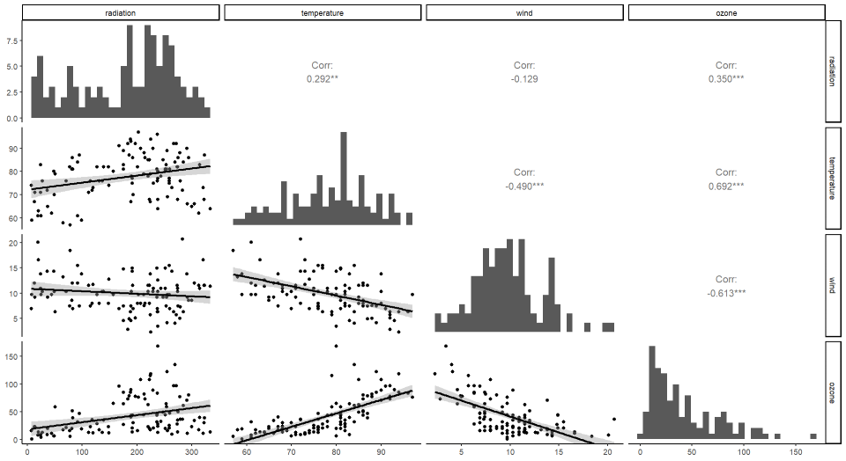
\includegraphics{images/scatter_matrix.png}\\
\strut \\

\paragraph{Multiplot Visualising ozone as the
response:}\label{multiplot-visualising-ozone-as-the-response}

\begin{Shaded}
\begin{Highlighting}[]
\CommentTok{\# Radiation}
\NormalTok{radiation\_plot }\OtherTok{\textless{}{-}}\NormalTok{ ozone }\SpecialCharTok{\%\textgreater{}\%}  \CommentTok{\# Choosing data frame and creating a plot with the pipe}
  \FunctionTok{ggplot}\NormalTok{(}\FunctionTok{aes}\NormalTok{(}\AttributeTok{x =}\NormalTok{ radiation, }\AttributeTok{y =}\NormalTok{ ozone)) }\SpecialCharTok{+}  \CommentTok{\# Setting variables for axis}
  \FunctionTok{geom\_point}\NormalTok{() }\SpecialCharTok{+}  \CommentTok{\# Scatterplot}
  \FunctionTok{labs}\NormalTok{(}\AttributeTok{x =} \StringTok{"Radiation (langleys)"}\NormalTok{, }\AttributeTok{y =} \StringTok{"Ozone (ppb)"}\NormalTok{) }\SpecialCharTok{+} \CommentTok{\# Axis Labels }
  \FunctionTok{theme\_classic}\NormalTok{()  }\CommentTok{\# Make background white}

\CommentTok{\# Temperature}
\NormalTok{temperature\_plot }\OtherTok{\textless{}{-}}\NormalTok{ ozone }\SpecialCharTok{\%\textgreater{}\%}  \CommentTok{\# Choosing data frame and creating a plot with the pipe}
  \FunctionTok{ggplot}\NormalTok{(}\FunctionTok{aes}\NormalTok{(}\AttributeTok{x =}\NormalTok{ temperature, }\AttributeTok{y =}\NormalTok{ ozone)) }\SpecialCharTok{+}  \CommentTok{\# Setting variables for axis}
  \FunctionTok{geom\_point}\NormalTok{() }\SpecialCharTok{+}  \CommentTok{\# Scatterplot}
  \FunctionTok{labs}\NormalTok{(}\AttributeTok{x =} \StringTok{"Temperature (farenheit)"}\NormalTok{, }\AttributeTok{y =} \StringTok{"Ozone (ppb)"}\NormalTok{) }\SpecialCharTok{+} \CommentTok{\# Axis Labels }
  \FunctionTok{theme\_classic}\NormalTok{()  }\CommentTok{\# Make background white}

\CommentTok{\# Wind speed}
\NormalTok{wind\_plot }\OtherTok{\textless{}{-}}\NormalTok{ ozone }\SpecialCharTok{\%\textgreater{}\%}  \CommentTok{\# Choosing data frame and creating a plot with the pipe}
  \FunctionTok{ggplot}\NormalTok{(}\FunctionTok{aes}\NormalTok{(}\AttributeTok{x =}\NormalTok{ wind, }\AttributeTok{y =}\NormalTok{ ozone)) }\SpecialCharTok{+}  \CommentTok{\# Setting variables for axis}
  \FunctionTok{geom\_point}\NormalTok{() }\SpecialCharTok{+}  \CommentTok{\# Scatterplot}
  \FunctionTok{labs}\NormalTok{(}\AttributeTok{x =} \StringTok{"Wind Speed (mph)"}\NormalTok{, }\AttributeTok{y =} \StringTok{"Ozone (ppb)"}\NormalTok{) }\SpecialCharTok{+} \CommentTok{\# Axis Labels }
  \FunctionTok{theme\_classic}\NormalTok{()  }\CommentTok{\# Make background white}


\FunctionTok{multiplot}\NormalTok{(radiation\_plot, wind\_plot, temperature\_plot, }\AttributeTok{cols =} \DecValTok{3}\NormalTok{)}
\end{Highlighting}
\end{Shaded}

The output is:\\
\strut \\
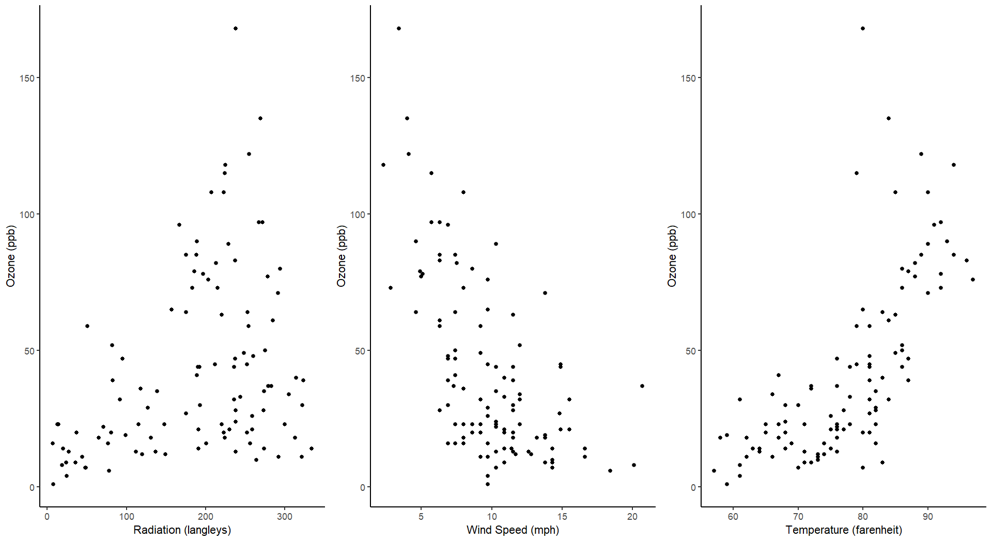
\includegraphics{images/ozone_relationships.png}\\

\paragraph{Discussion of findings:}\label{discussion-of-findings}

Starting with the relationship between radiation and ozone, there
appears to be a slight positive correlation. This is supported by the
correlation coefficient of 0.35 seen in the scatter matrix which
confirms a weak positive correlation. Furthermore, through visual
assessment, it appears that the effect of radiation on ozone appears to
be more volatile at higher radiations and suggest that any linearity
could be heteroscedsatic with more variation in residuals at higher
radiations.\\

Moving onto the relationship between ozone and windspeed, there appears
to be a negative correlation (-0.613). However, the strongest
correlation is between temperature and ozone which is positive and has a
correlation coefficient of 0.692.\\

Judging by the correlation coefficients, there does not appear to be any
extreme co-linearity between any of the variables despite the fact that
wind speed and temperature are almost certainly non-independent.\\

\hfill\break
\hfill\break
\hfill\break

\subsection{Question 7b}\label{question-7b}

\paragraph{Creating the linear model}\label{creating-the-linear-model}

\begin{Shaded}
\begin{Highlighting}[]
\NormalTok{model }\OtherTok{\textless{}{-}} \FunctionTok{lm}\NormalTok{ (ozone }\SpecialCharTok{\textasciitilde{}}\NormalTok{ temperature }\SpecialCharTok{+}\NormalTok{ wind }\SpecialCharTok{+}\NormalTok{ radiation, }\AttributeTok{data =}\NormalTok{ ozone)  }\CommentTok{\# Response and fixed effects}
\FunctionTok{summary}\NormalTok{(model)}
\end{Highlighting}
\end{Shaded}

The summary of the model which including the three fixed explanatory
effects highlights the extent of their relationship with ozone (ppb).
Firstly, the effect of temperature is positive as expected; the estimate
is 1.6 which means that for every increase in 1 degrees Fahrenheit there
is an associated increase in ozone of 1.6 ppb. This supports the initial
expectations. This relationship is statistically significant at the 0.05
significance threshold (used for all future analyses), (p
\textless0.0001). This was the most significant result which I also
predicted given the initial visualisation.

For wind speed, the estimate of -3.39 also supports the negative
correlations and coefficients observed din question 7a. The p-value here
is also very significant (p = \textless0.0001).

Finally, and also unexpectedly, the effect of radiation on ozone was
also significant (p \textless{} 0.05). While I had identified the weak
positive relationship beforehand, which is compounded by the estimate
for radiation's effect of 0.06, I had not expected this weak
relationship to render a statistically significant finding.

It should be noted that I have not used a linear mixed effects model.
However, it could be argued that wind temperature and radiation's effect
on the ozone could depend on each variables levels, thus making the
current model too simple. Furthermore to test whether the models
assumptions have been violated or not, I will check the diagnostic
plots.

\paragraph{Model Validity Checks}\label{model-validity-checks}

I generate the diagnostic plots by:

\begin{Shaded}
\begin{Highlighting}[]
\FunctionTok{par}\NormalTok{(}\AttributeTok{mfrow =} \FunctionTok{c}\NormalTok{(}\DecValTok{2}\NormalTok{, }\DecValTok{2}\NormalTok{))}
\FunctionTok{plot}\NormalTok{(model)}
\end{Highlighting}
\end{Shaded}

\hfill\break
This gives:\\
\strut \\
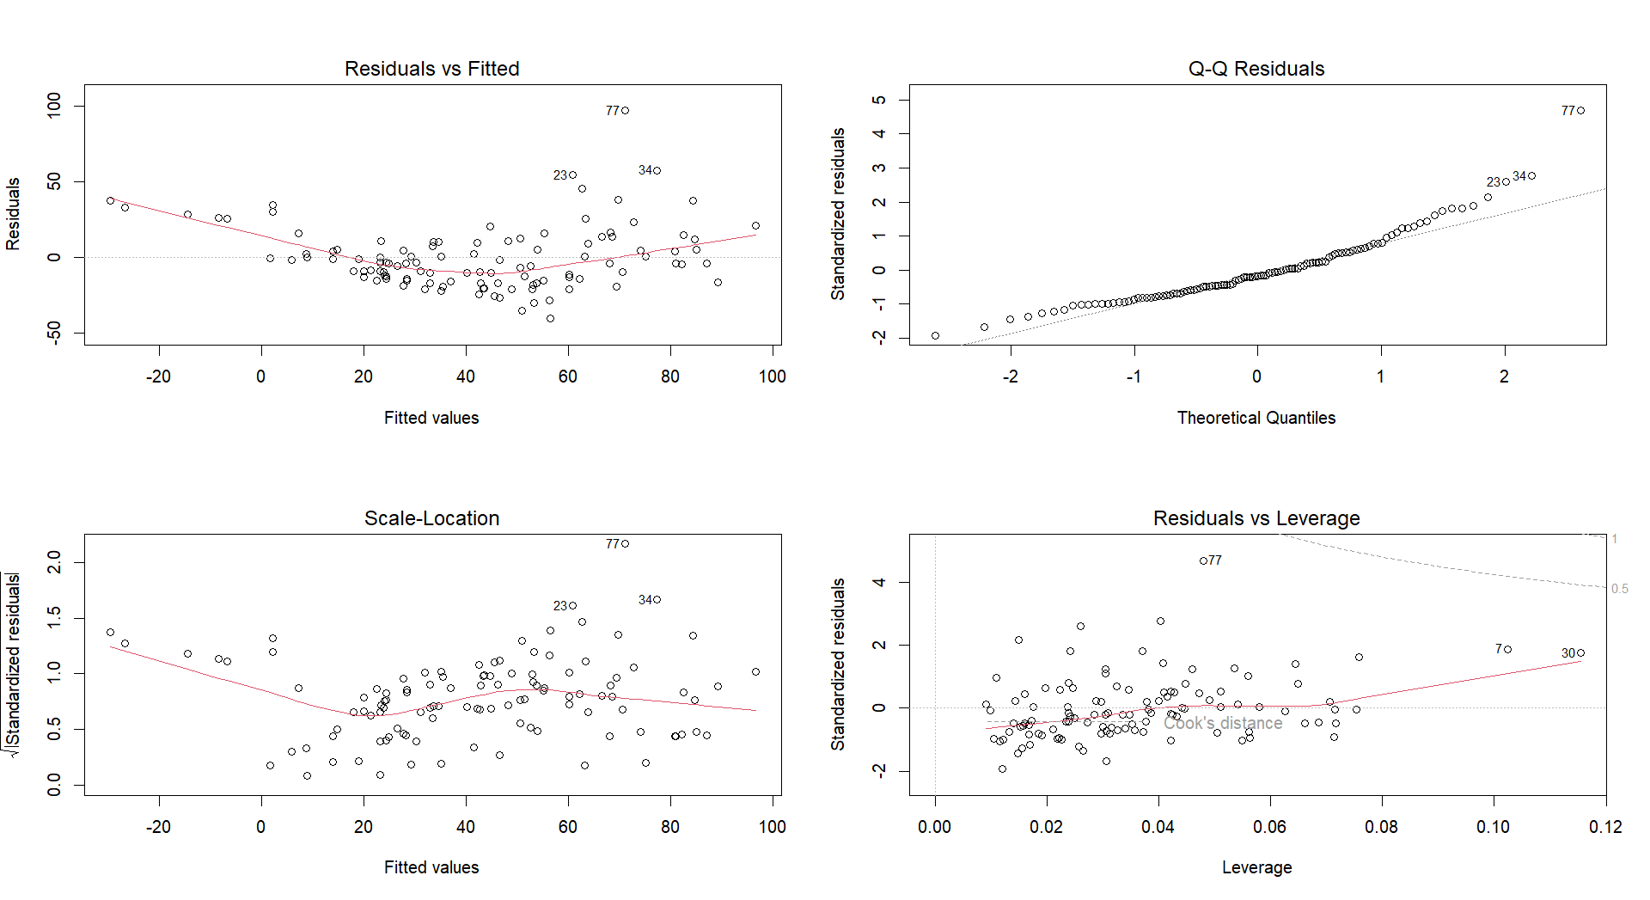
\includegraphics{images/diagnostic_plots.png}\\
\strut \\
The diagnostic plot give a host of insights into whether the model
assumptions have been violated. Firstly, the `Residuals vs Fitted'
values reveal that there is a level of heteroscedasticity in the data.
It shows that the spread of residuals across different levels of the
fitted values is inconsistent. Therefore the assumption that they are
even (the assumption of homoscedasticity) has been violated. In
particular, there appears to be a more erratic spread of residuals at
the extremes of the fitted values. A similar interpretation can be made
for the `Scale-Location' plot.

Next, the assumption of normality in the residuals distribution has also
been violated. This can be seen in the Q-Q plot whereby a number of
residuals deviate from the expected normal distribution (along the
dotted line). This is most apparent when looking at the data point from
the 77th day.

Finally, the `Residuals vs Leverage' diagnostic plot shows that the
there are no residuals that have a extreme and noteworthy effect on the
conclusions. Generally, a Cook's score that exceeds 1 is regarded as
extreme leverage and yet none exceed 0.5. In turn, I can conclude that
there are no residuals with extreme leverage that could have a
disproportionate influence on the model outputs

In conclusion, the model's reliability is limited in some respect.
Namely, the lack of homoscedasticity and normality in the residuals
limits the validity of inferring the results of the model.\\
\strut \\
\strut \\

\subsection{Question 7c}\label{question-7c}

\begin{Shaded}
\begin{Highlighting}[]
\NormalTok{model\_2 }\OtherTok{\textless{}{-}} \FunctionTok{lm}\NormalTok{ (}\FunctionTok{log}\NormalTok{(ozone) }\SpecialCharTok{\textasciitilde{}} \FunctionTok{log}\NormalTok{(temperature) }\SpecialCharTok{+} \FunctionTok{log}\NormalTok{(wind) }\SpecialCharTok{+} \FunctionTok{log}\NormalTok{(radiation), }\AttributeTok{data =}\NormalTok{ ozone)  }\CommentTok{\# Log{-}transform variables}
\FunctionTok{summary}\NormalTok{(model\_2) }\CommentTok{\# Model summary}
\end{Highlighting}
\end{Shaded}

Starting with the model outputs, it is clear to see that
log-transforming the response and explanatory effects has affected the
coefficients and the corresponding p-values:\\
\strut \\
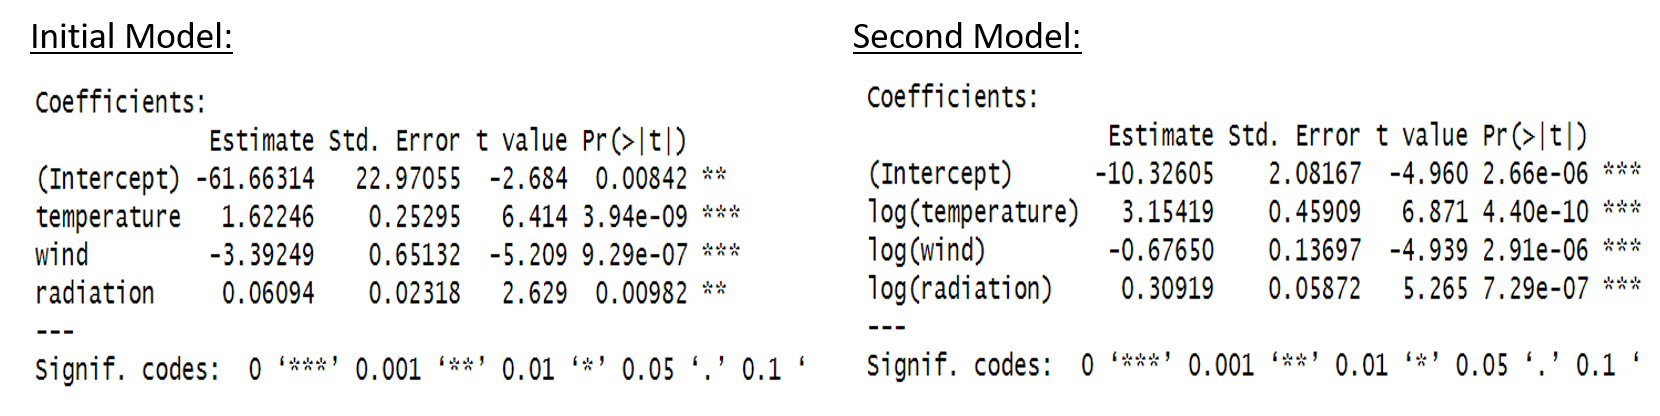
\includegraphics{images/coefficients_comparison.png}\\
\strut \\

Firstly, the modelled effect of wind speed on ozone has been greatly
reduced. The coefficent is -0.68 which means that the second model
predicts for every 1 mph increase in wind speed, there is a
\textasciitilde2.27 smaller change in the ozone compared to the first
model. This is undoubtedly caused by the log transformation. Earlier, I
identified data point 77 as a clear outlier. Upon looking at the data, I
can see that this data point contains the highest ozone recording (168
ppb) and the second lowest wind speed (3.4 mph). The log transformation
would have made this raw data less extreme relative to the rest of the
data and therefore the modelled effect of wind speed on ozone has been
largely suppressed hence the less extreme coefficient and p-value
(2.91e-06 compared to the first models p value of 9.29-07).

In contrast, the log transformation has heightened the perceived impact
of radiation and temperature in comparison to the first model with
coefficients coefficients increasing from 0.06 to 0.31 and 1.62 to 3.15,
respectively. In turn, the model successfully explains more of the
random varaition in the data (noise) compared to the previous model. The
most likely explanation for this is that the transformation has made the
data more linear; it has made the extreme residual values (discussed in
the previous question) less extreme relative to the rest of the data.
This is evidenced by assessing the diagnostic plots:\\
\strut \\

\begin{Shaded}
\begin{Highlighting}[]
\FunctionTok{par}\NormalTok{(}\AttributeTok{mfrow =} \FunctionTok{c}\NormalTok{(}\DecValTok{2}\NormalTok{, }\DecValTok{1}\NormalTok{))}
\FunctionTok{plot}\NormalTok{(model\_2)}
\end{Highlighting}
\end{Shaded}

\hfill\break
\hfill\break
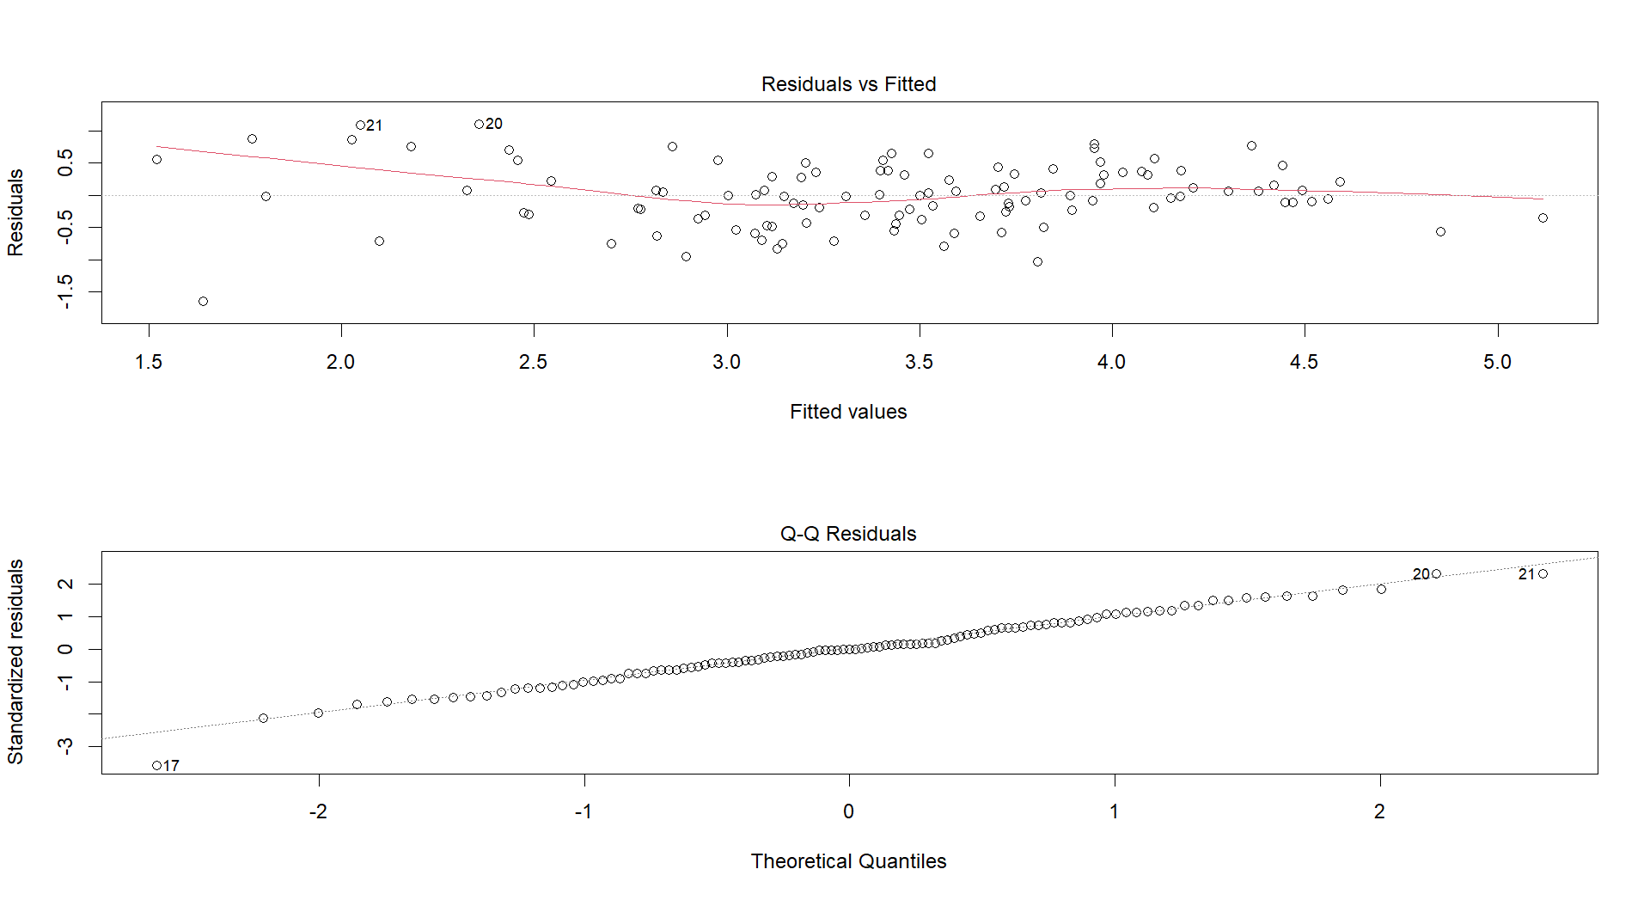
\includegraphics{images/7c_diagnostic_plots.png}\\
\strut \\

In comparison to the former models diagnostic plot, this `Residuals vs
Fitted' plot highlights a huge amelioration in the extent of
heteroscedasticity in the data. Now the residuals are much more evenly
distributed around the flat x axis line. This means that the variance of
the residuals is more consistent and that the assumption of
homoscedasticity has not been violated to the same extent as before.
Furthermore, the linearity of the residuals is much better as can be
seen in the Q-Q plot; this means that the residuals follow the normal
distribution assumed of linear models. While I have not used statistical
tests to confirm whether the model assumptions have been met such as the
Bartlett test for homoscedasticity and the Shapiro Wilks for normality,
I can at least confirm through visual assessment of the diagnostic plot
that the transformations have made the data in the second model more
appropriate for a linear model.

\end{document}
